\documentclass{article}
\usepackage{amsmath}
\usepackage{amssymb}
\usepackage{graphicx}
\usepackage{caption}
\usepackage{float}
\usepackage{subcaption}
\usepackage{pdflscape}
\usepackage[table,xcdraw]{xcolor}

\author{Cláudio Ferreira Carneiro - RA 263796}
\title{EFC 2}
\begin{document}
    \maketitle
    \pagenumbering{gobble}
    \newpage
    \pagenumbering{arabic}
    \section[]{Parte 1 –Classificação binária}
    O código referente às atividades se encontra no repositório:
    
    https://github.com/carneirofc/IA006.git\linebreak
    \subsection[]{a) Características dos atributos de entrada}
        Os histogramas dos atributos em sua forma original são apresentados nas figuras \ref{fig:a_hist_1},
        \ref{fig:a_hist_2} e \ref{fig:a_hist_3}. A correlação dos atributos é apresentada
        na forma de um \textit{heatmap} \ref{fig:a_corr_heat} e por gráficos de dispersão \ref{fig:a_corr_scatter}
        (na diagonal principal é exibido o histograma do atributo).
        Percebe-se que determinados atributos apresentam alto grau de correlação.
        
        \begin{figure}[H]
            \begin{subfigure}{.5\textwidth}
                \centering
                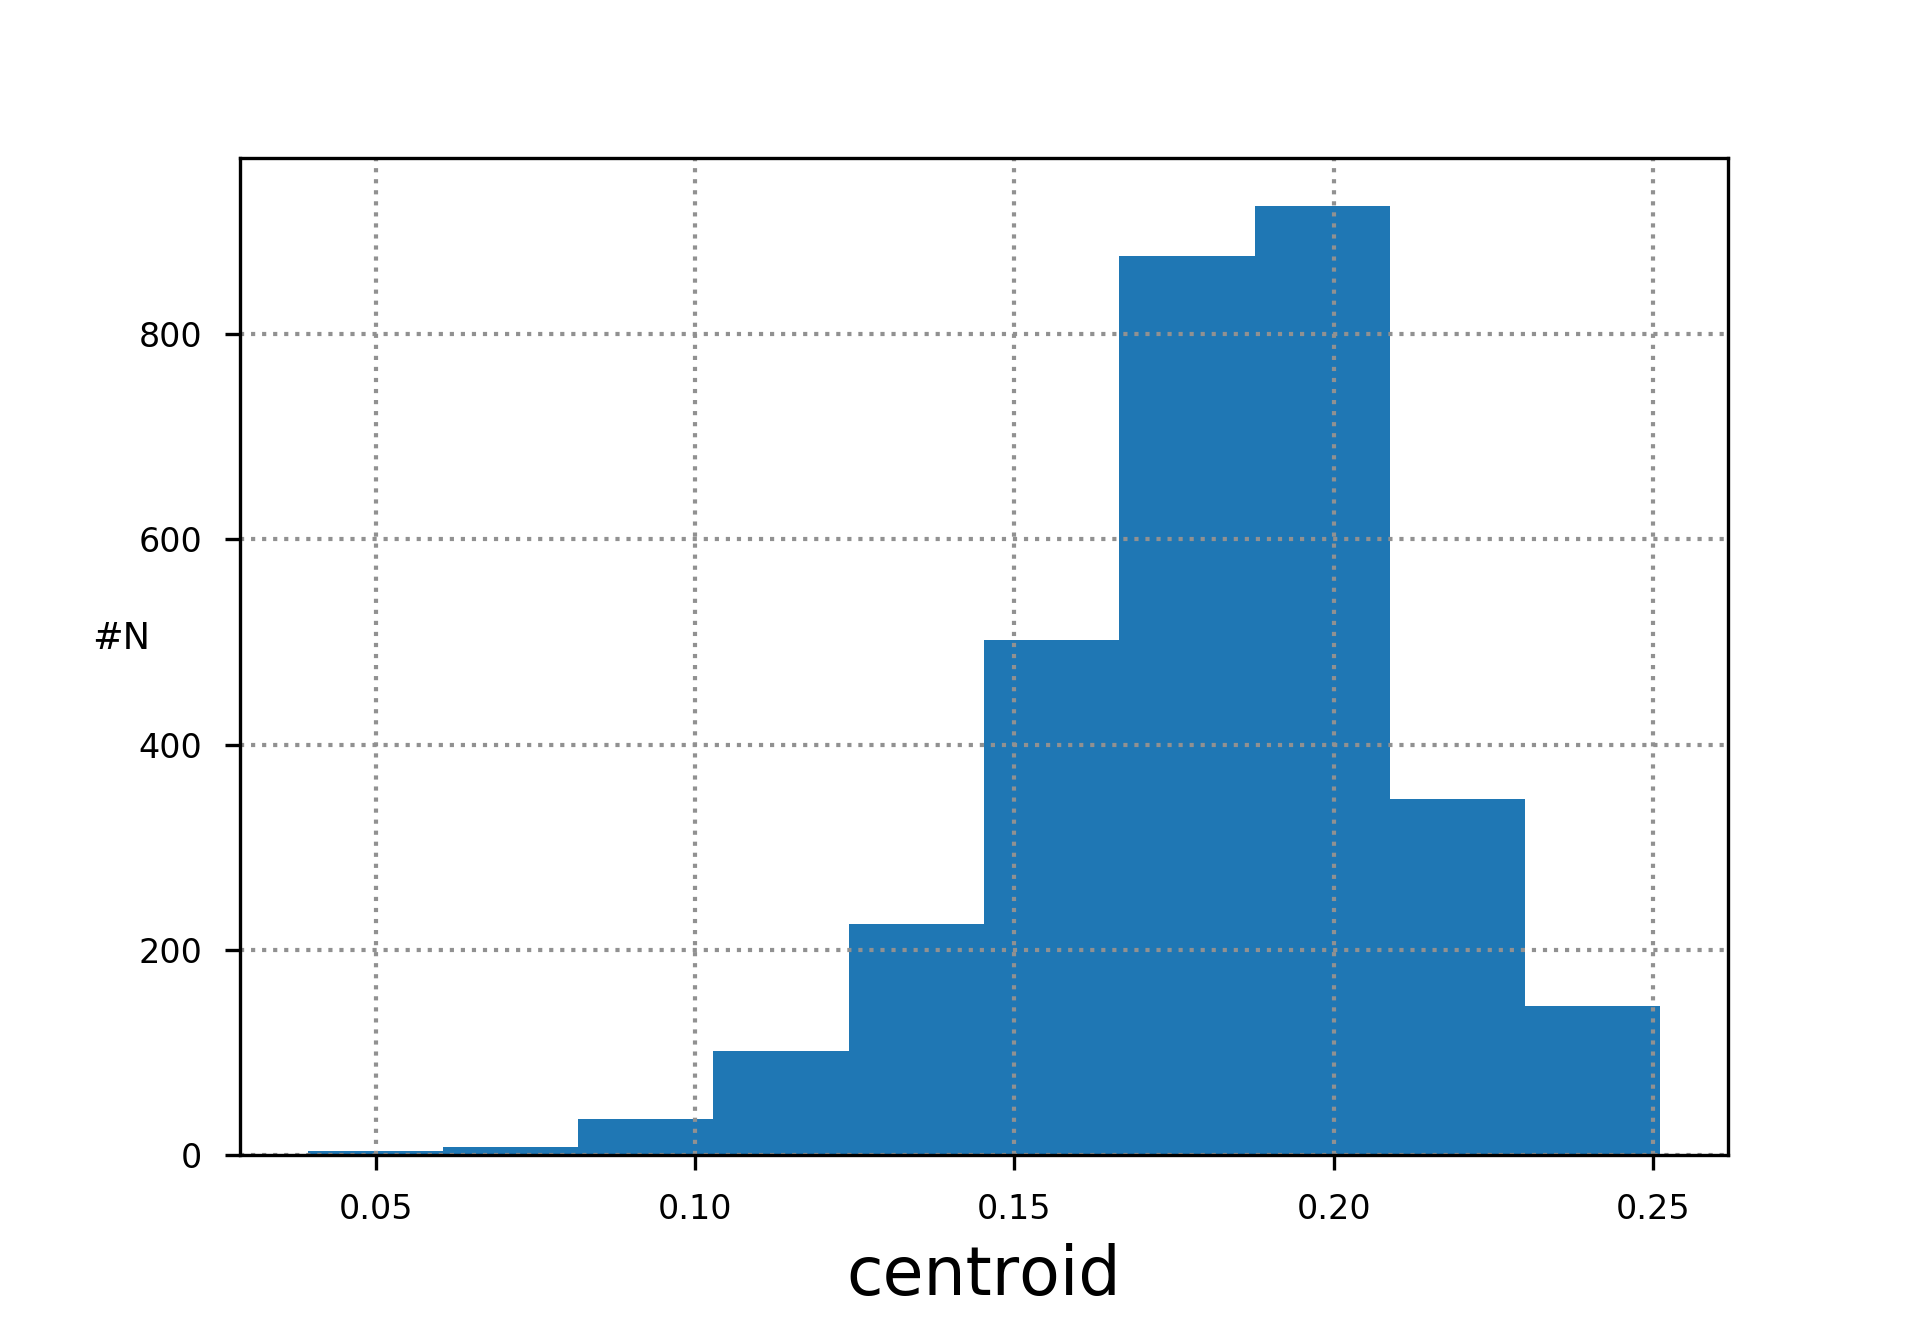
\includegraphics[width=.8\linewidth]{img1/data_histcentroid.png}
                \caption{Centroid}
            \end{subfigure}%
            \begin{subfigure}{.5\textwidth}
                \centering
                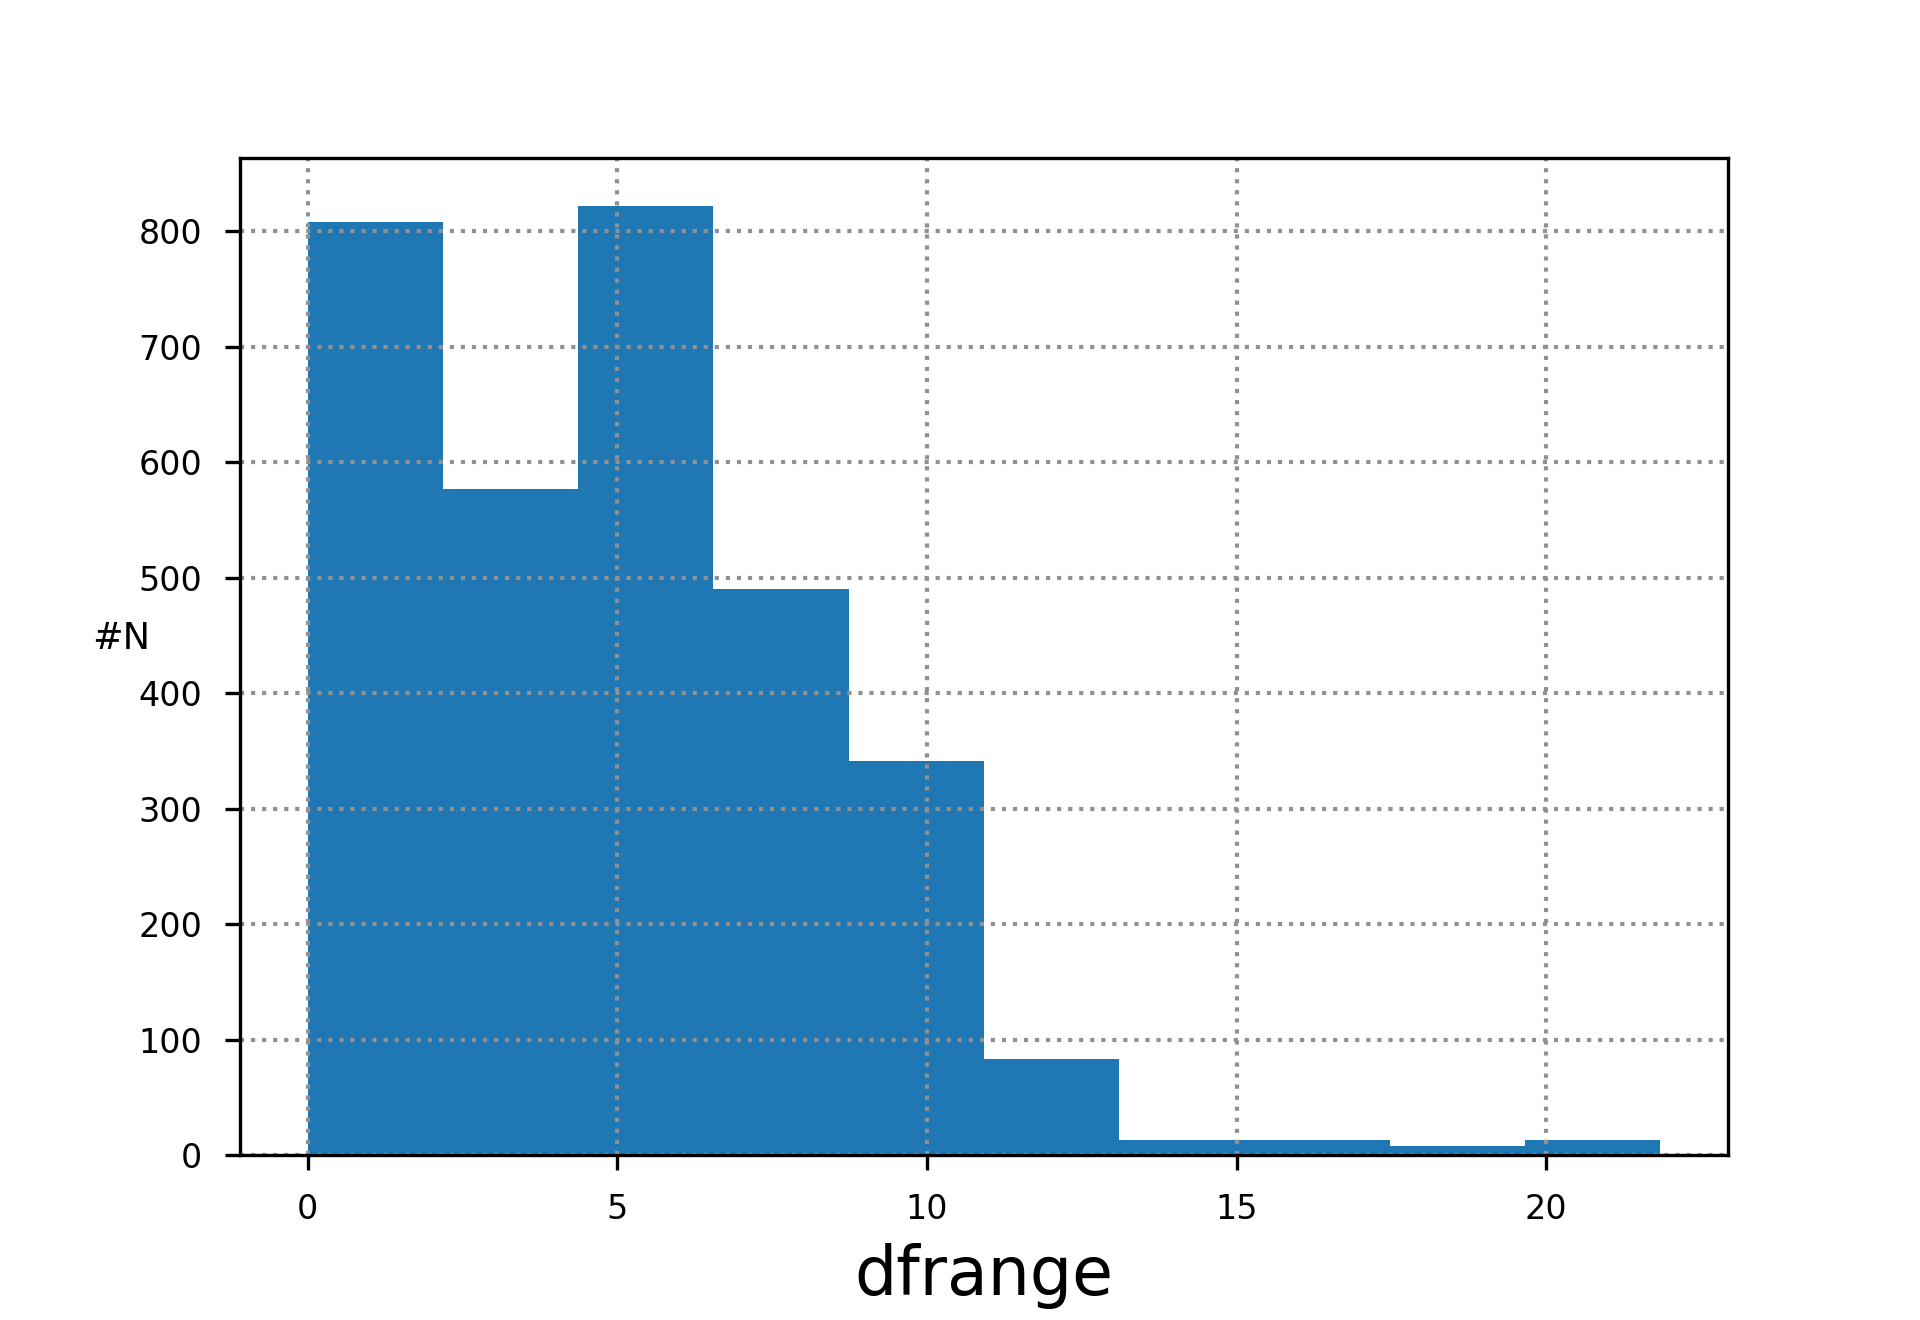
\includegraphics[width=.8\linewidth]{img1/data_histdfrange.png}
                \caption{F-Range}
            \end{subfigure}
            \begin{subfigure}{.5\textwidth}
                \centering
                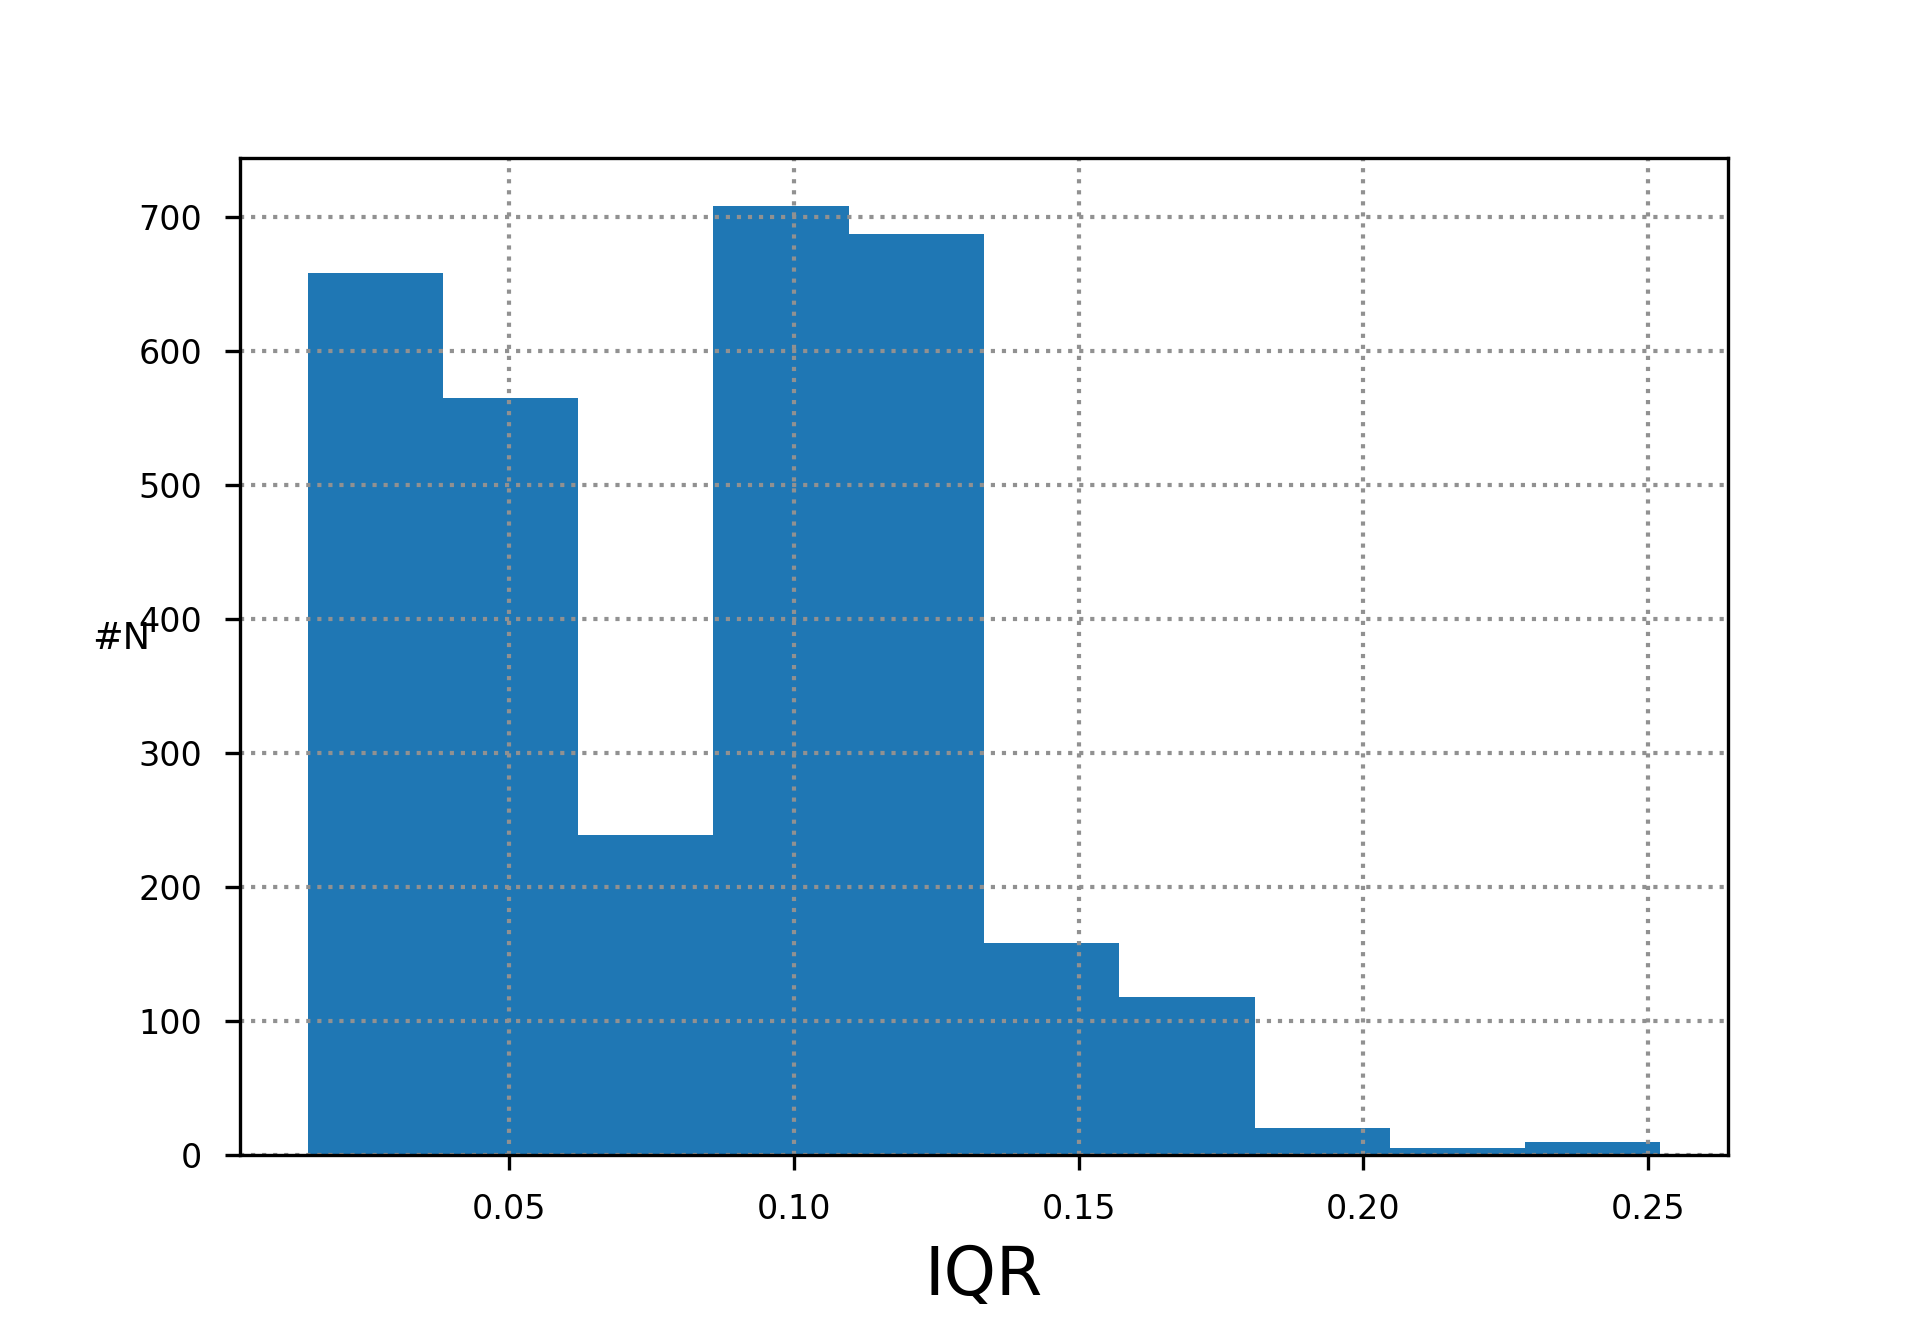
\includegraphics[width=.8\linewidth]{img1/data_histIQR.png}
                \caption{IQR}
            \end{subfigure}
            \begin{subfigure}{.5\textwidth}
                \centering
                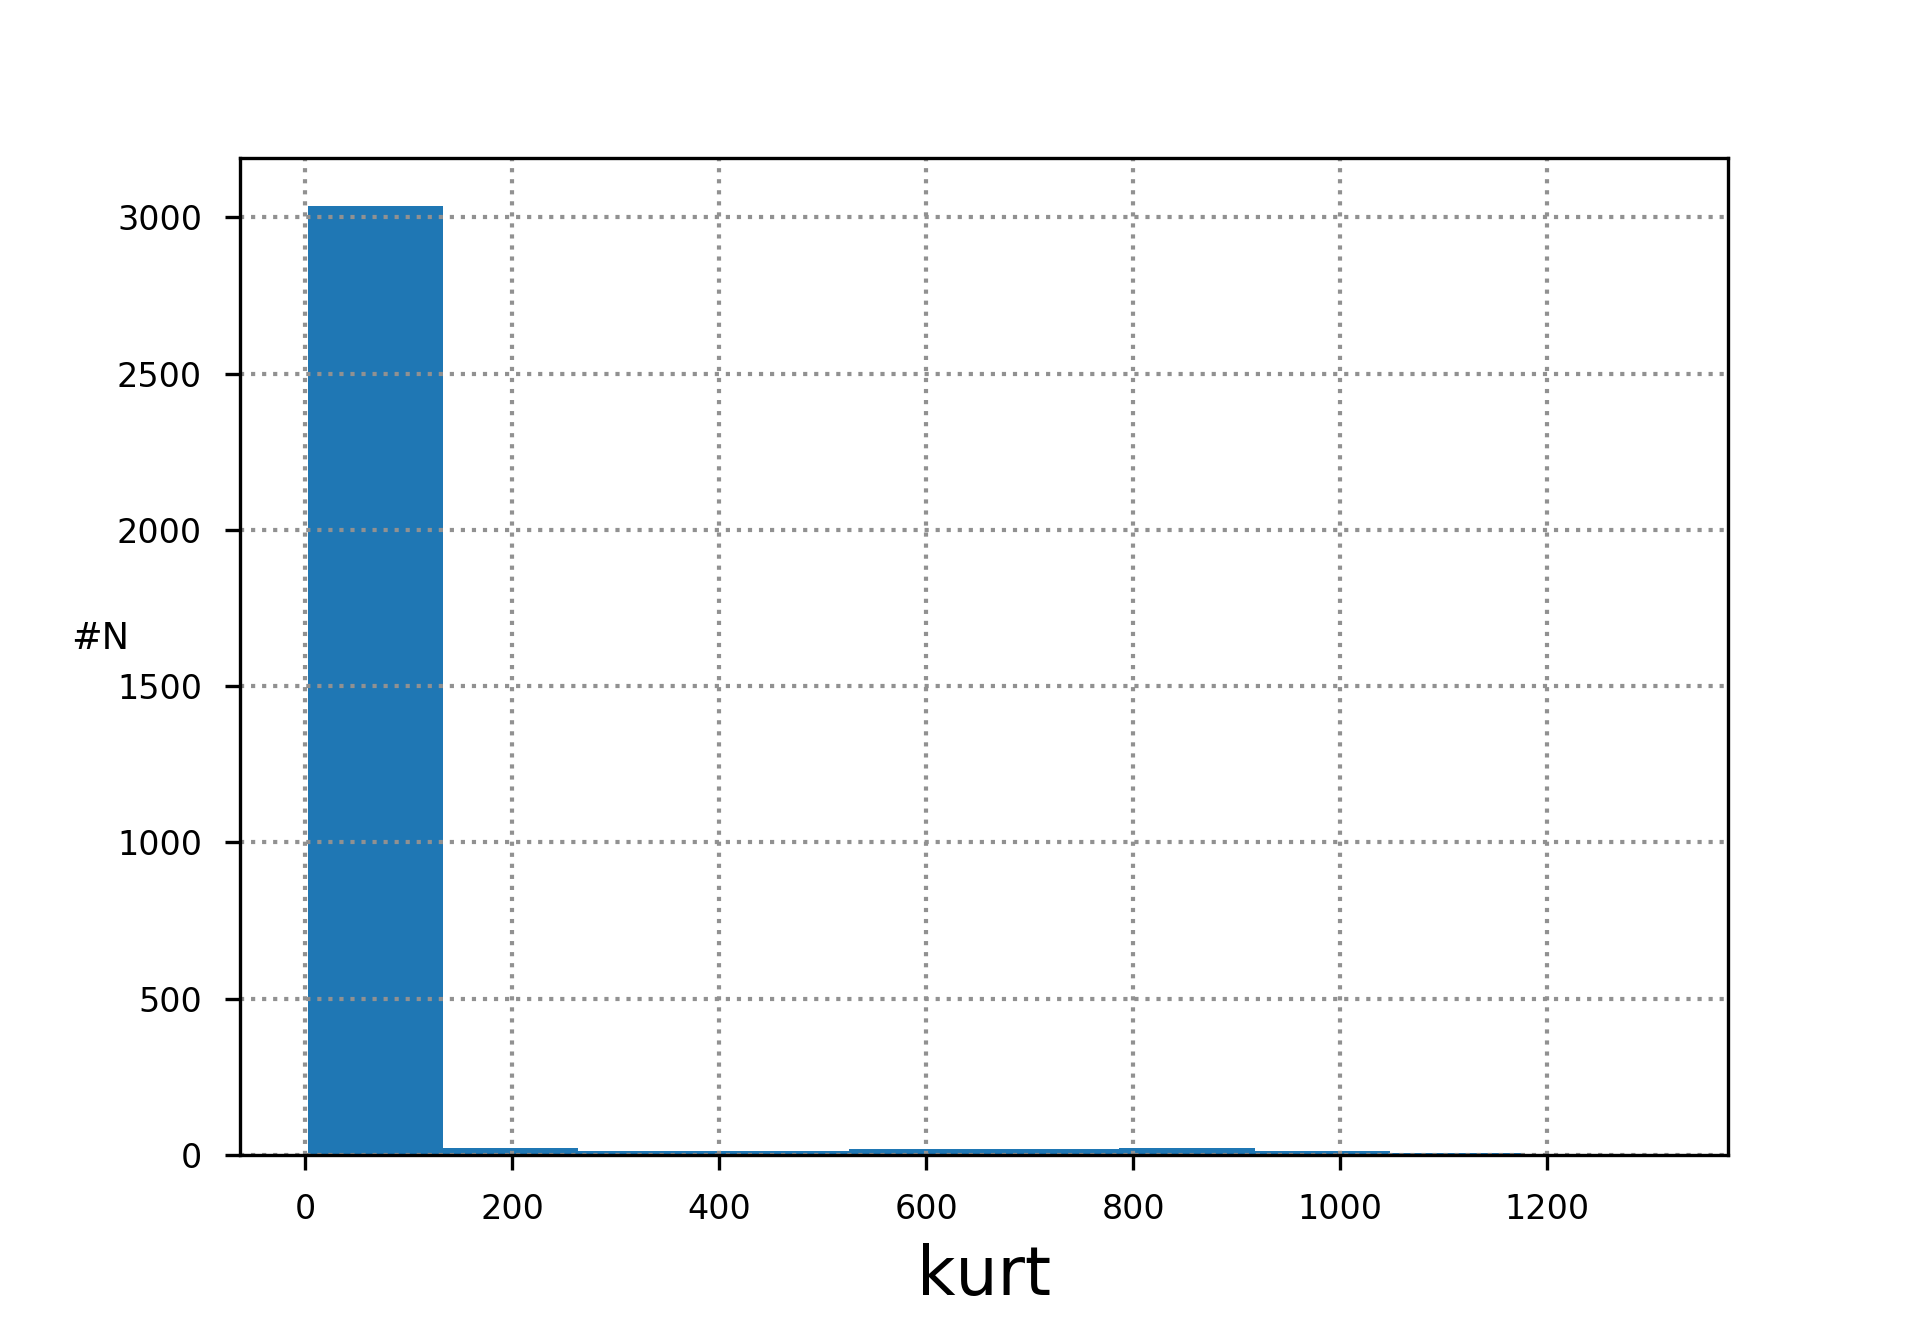
\includegraphics[width=.8\linewidth]{img1/data_histkurt.png}
                \caption{Kurt}
            \end{subfigure}
            \begin{subfigure}{.5\textwidth}
                \centering
                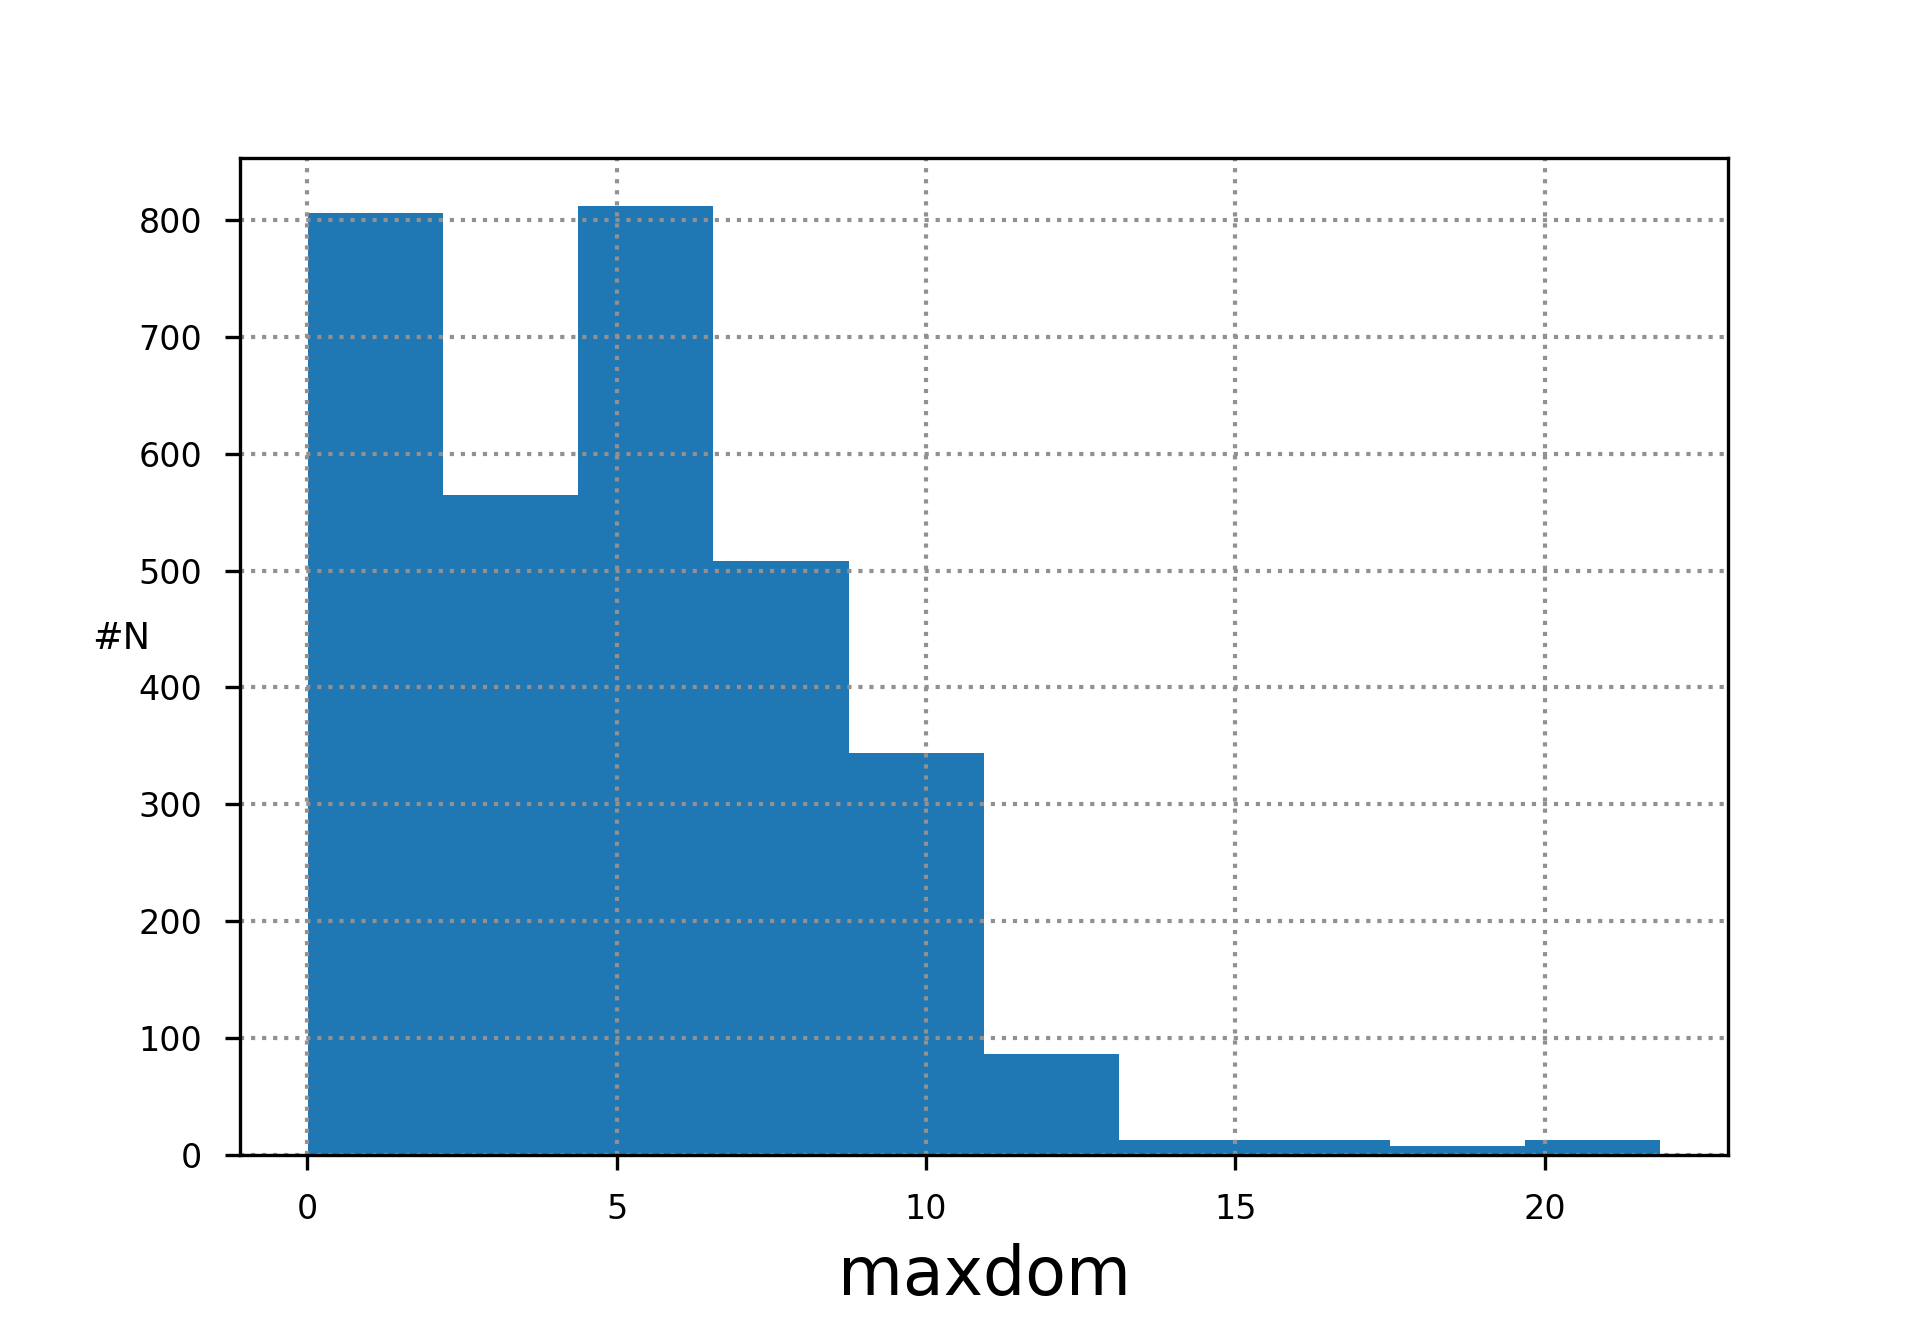
\includegraphics[width=.8\linewidth]{img1/data_histmaxdom.png}
                \caption{Max dom}
            \end{subfigure}
            \begin{subfigure}{.5\textwidth}
                \centering
                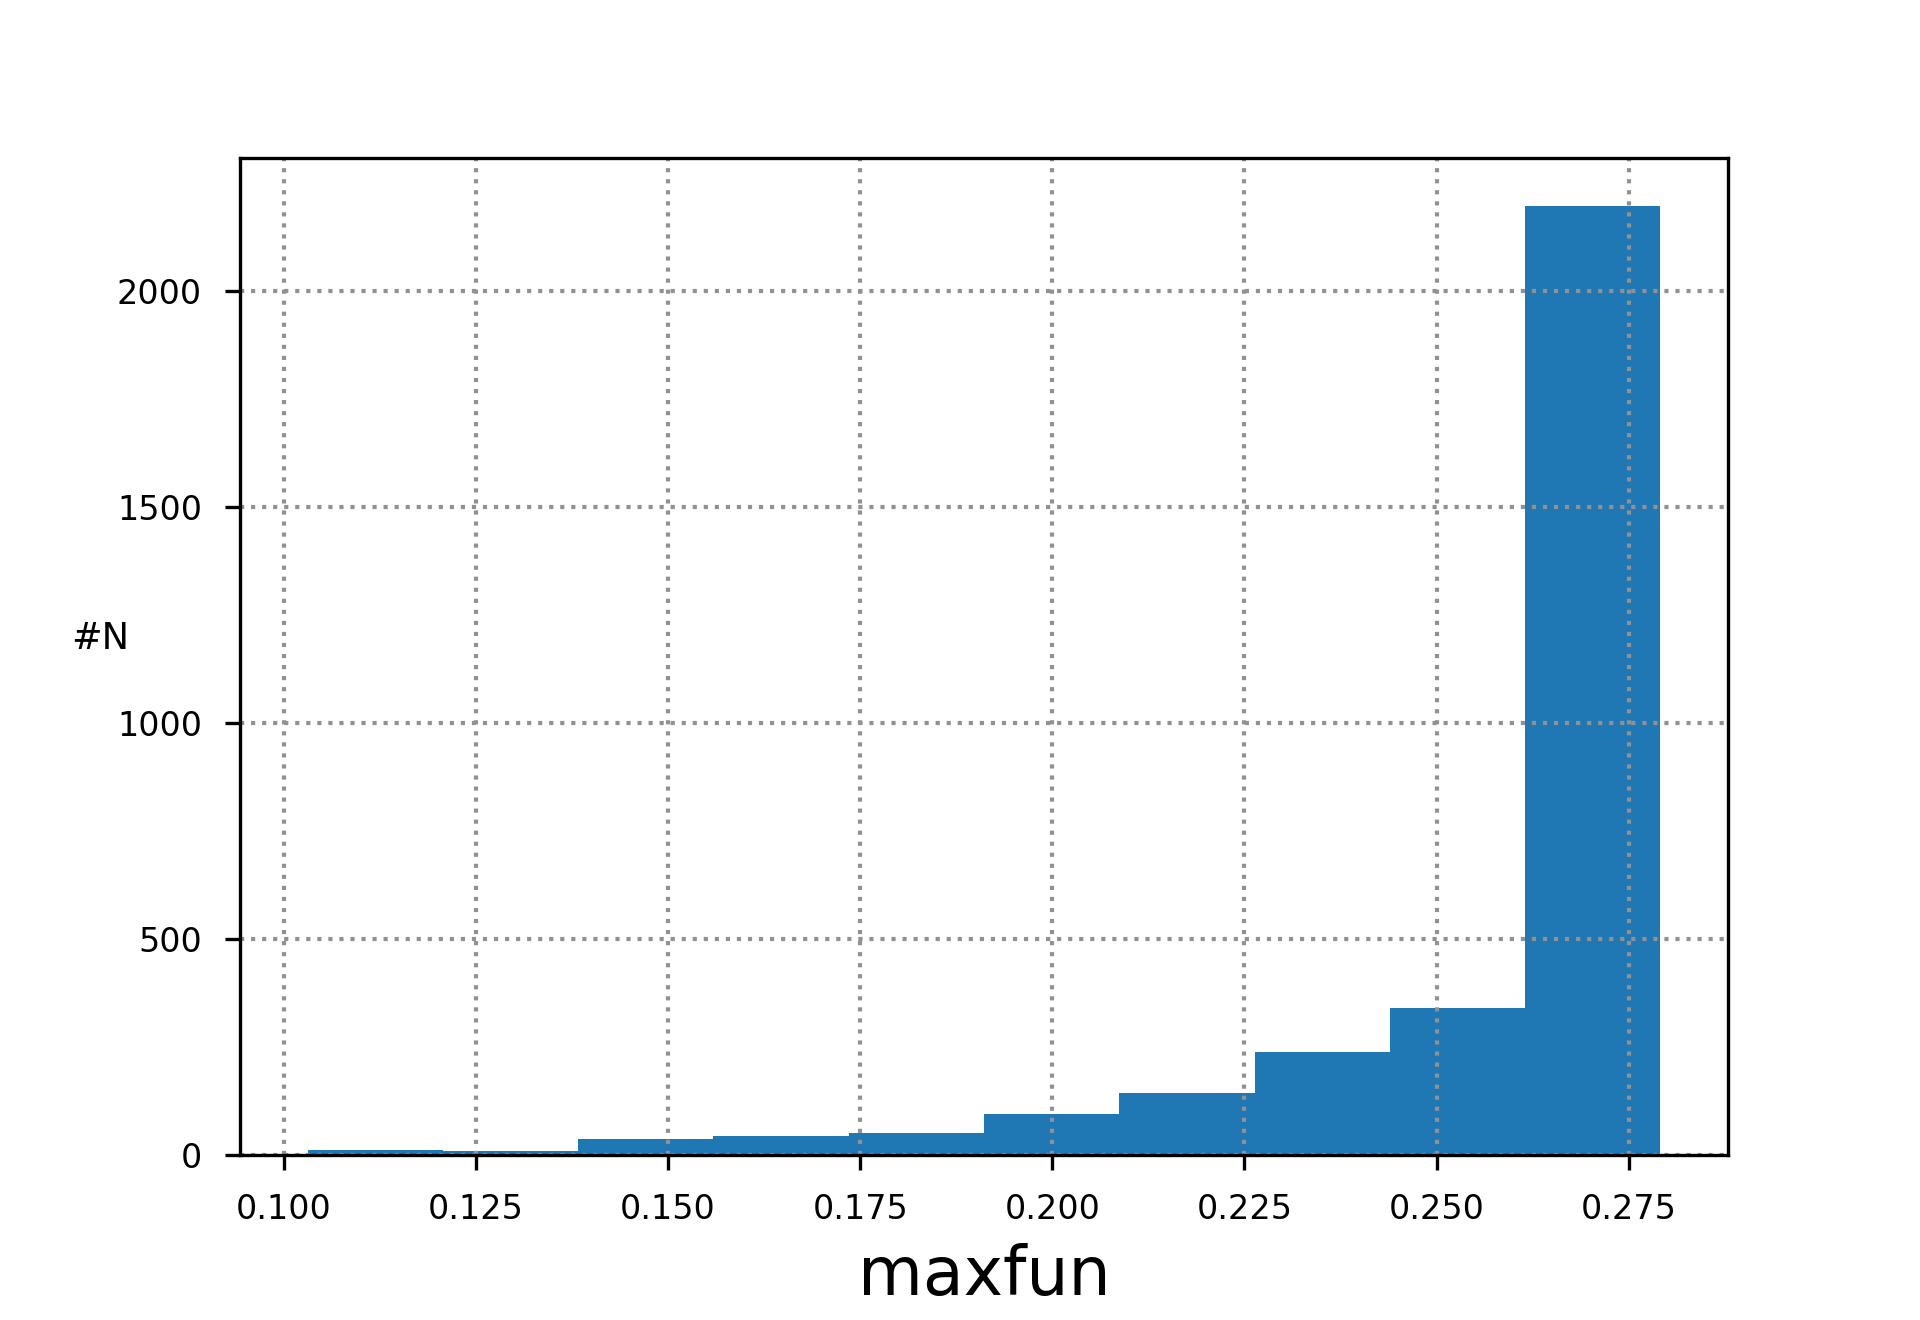
\includegraphics[width=.8\linewidth]{img1/data_histmaxfun.png}
                \caption{Max fun}
            \end{subfigure}
            \begin{subfigure}{.5\textwidth}
                \centering
                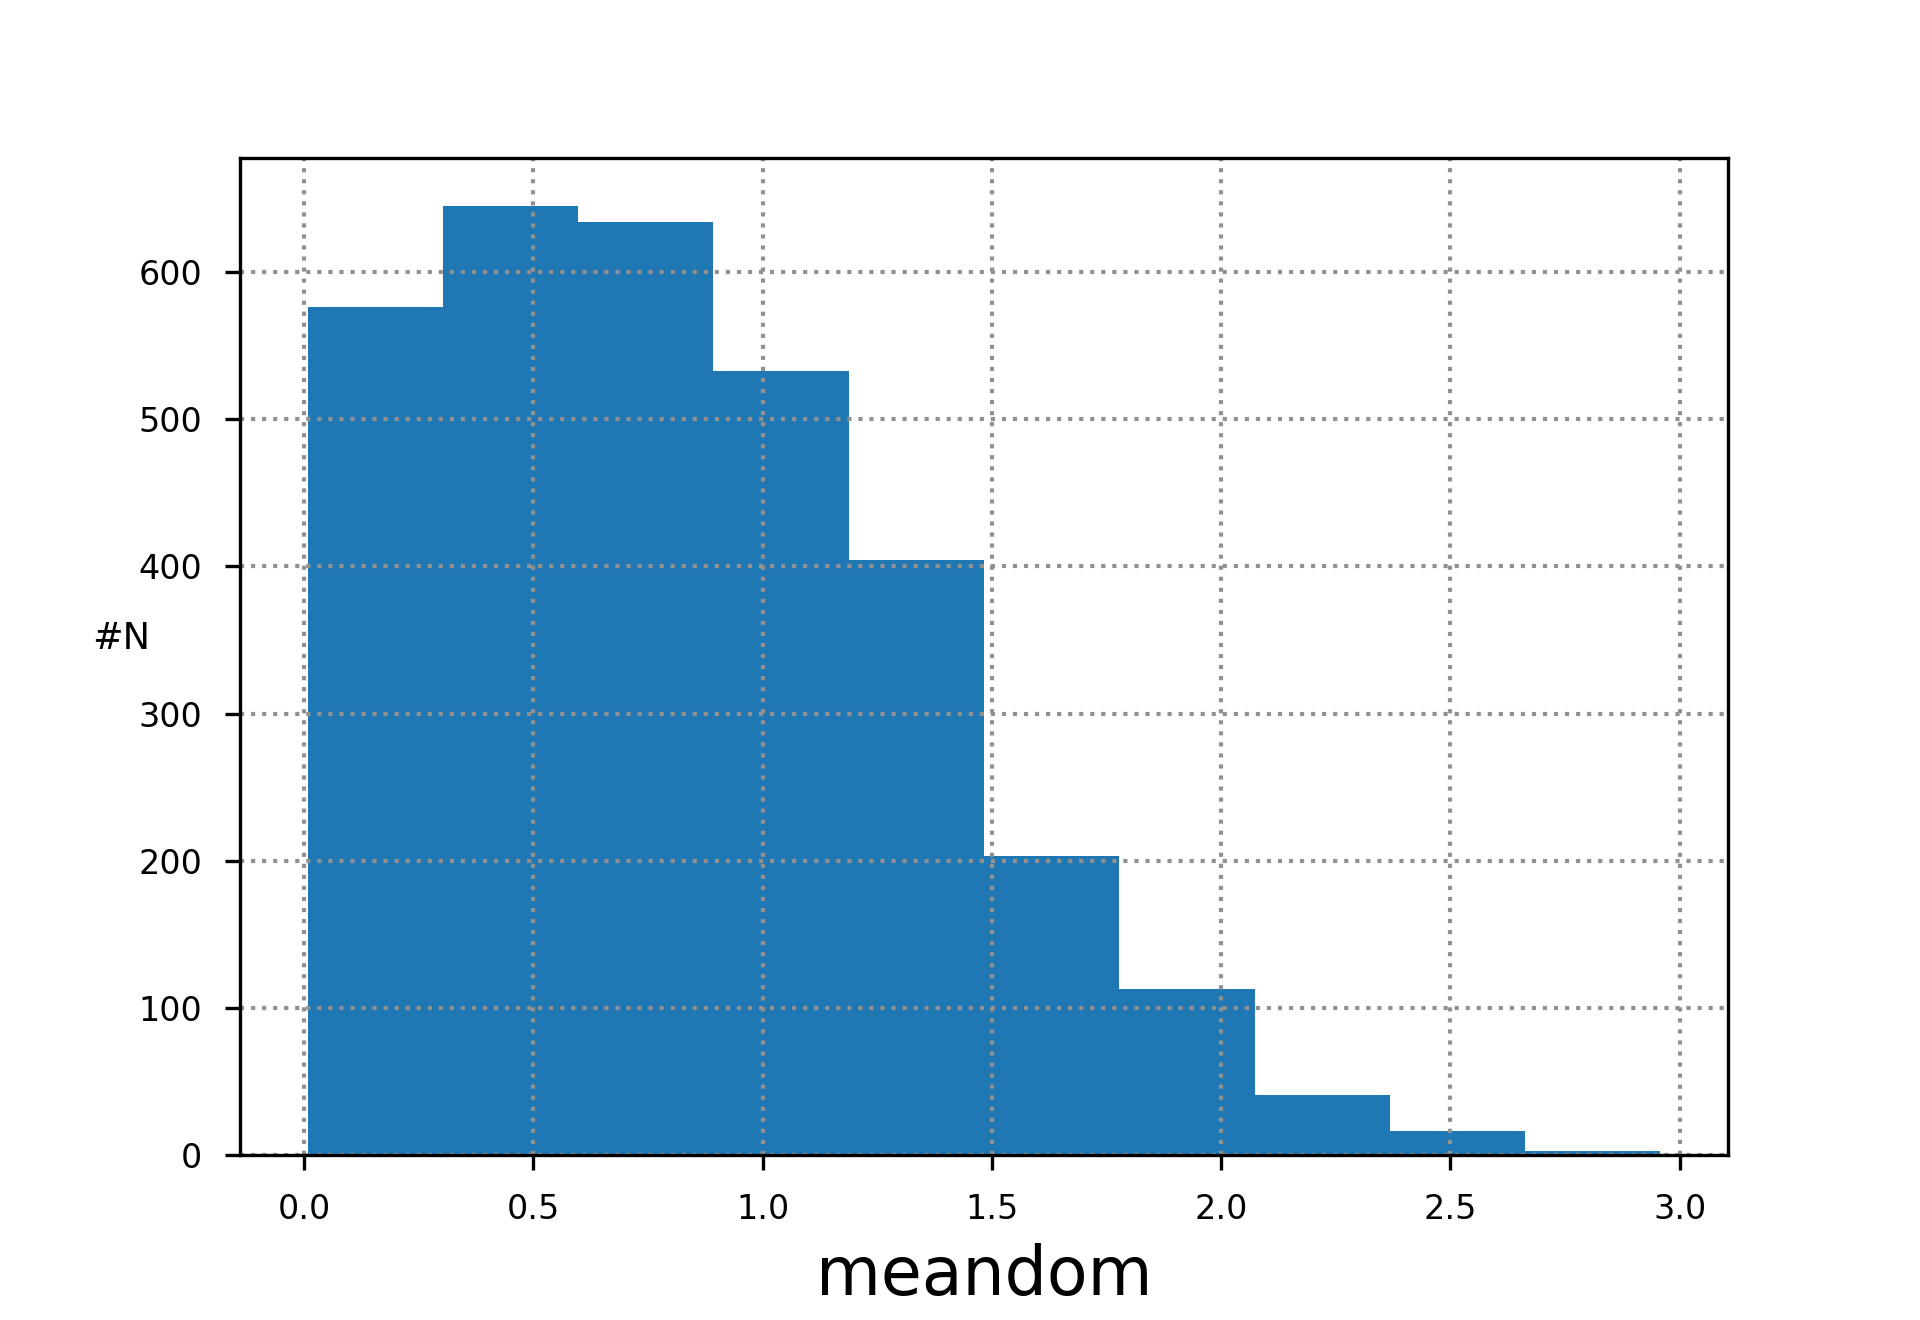
\includegraphics[width=.8\linewidth]{img1/data_histmeandom.png}
                \caption{Mean dom}
            \end{subfigure}
            \begin{subfigure}{.5\textwidth}
                \centering
                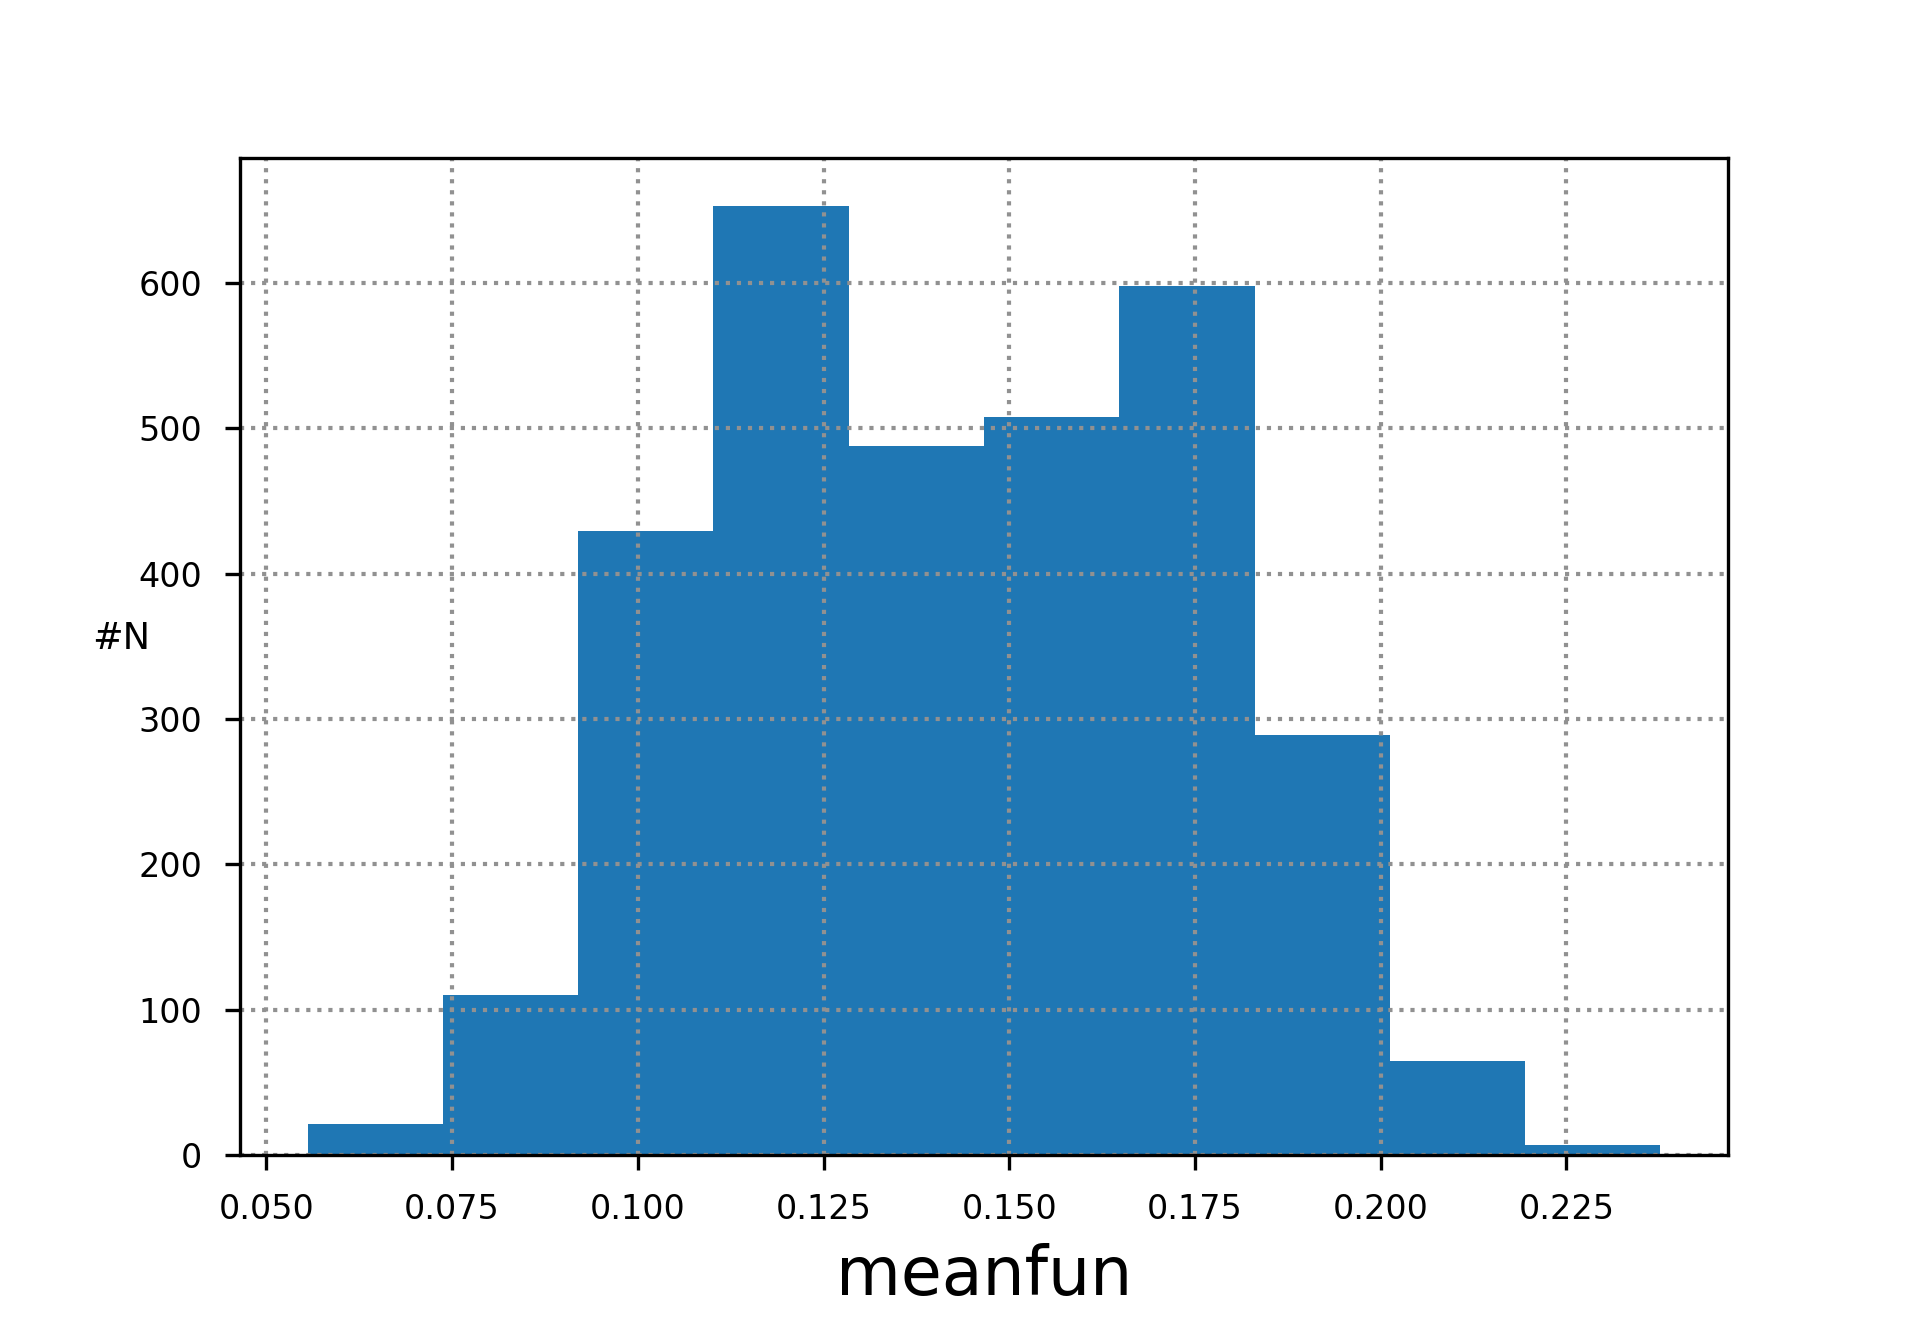
\includegraphics[width=.8\linewidth]{img1/data_histmeanfun.png}
                \caption{Mean fun}
            \end{subfigure}
        \caption{Classificação binária: Histograma dos atributos (1)}
        \label{fig:a_hist_1}
        \end{figure}
        \begin{figure}[H]
            \begin{subfigure}{.5\textwidth}
                \centering
                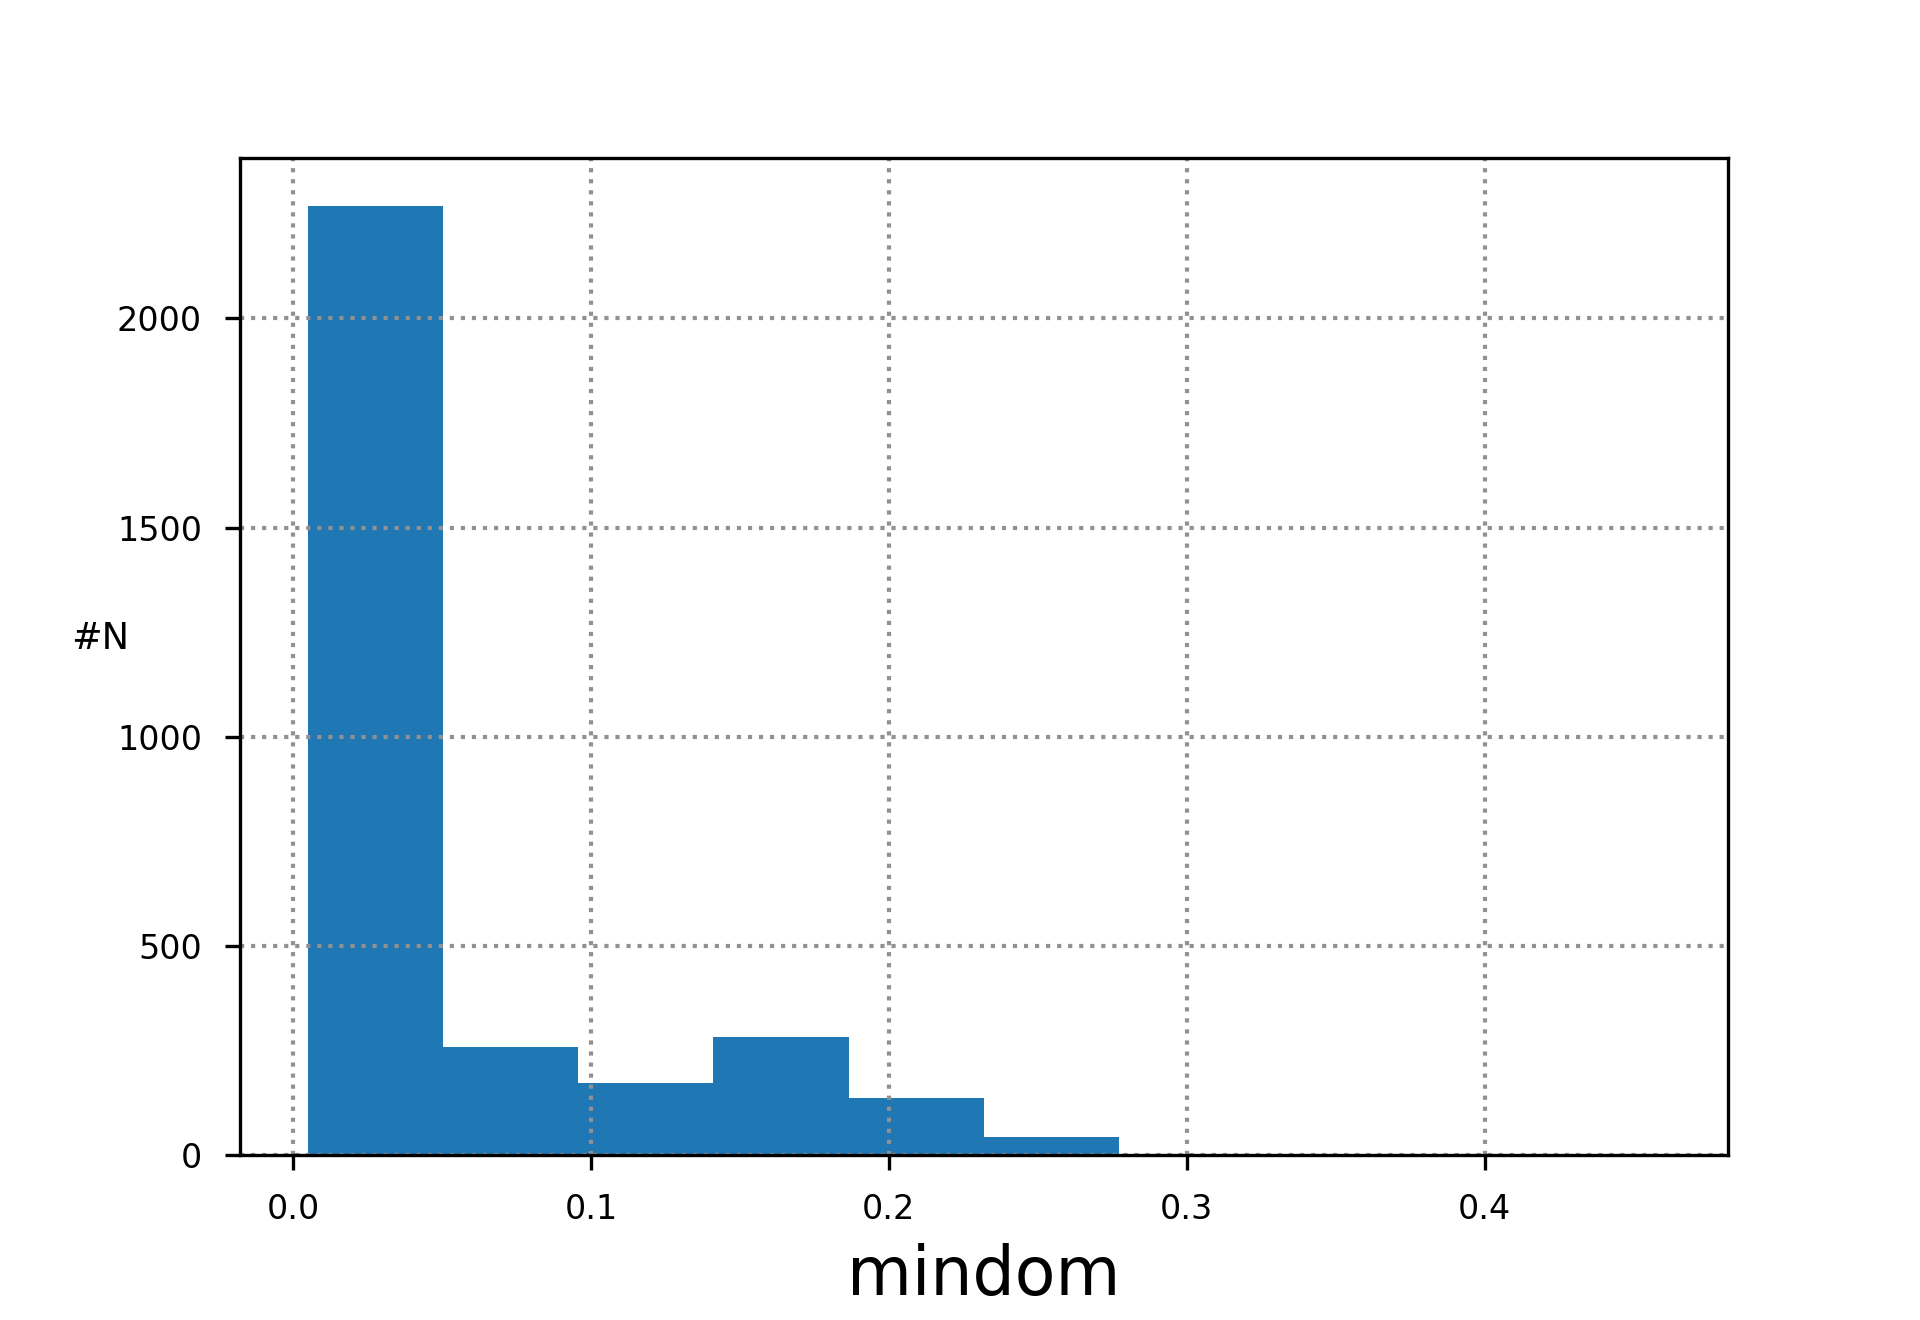
\includegraphics[width=.8\linewidth]{img1/data_histmindom.png}
                \caption{Min dom}
            \end{subfigure}
            \begin{subfigure}{.5\textwidth}
                \centering
                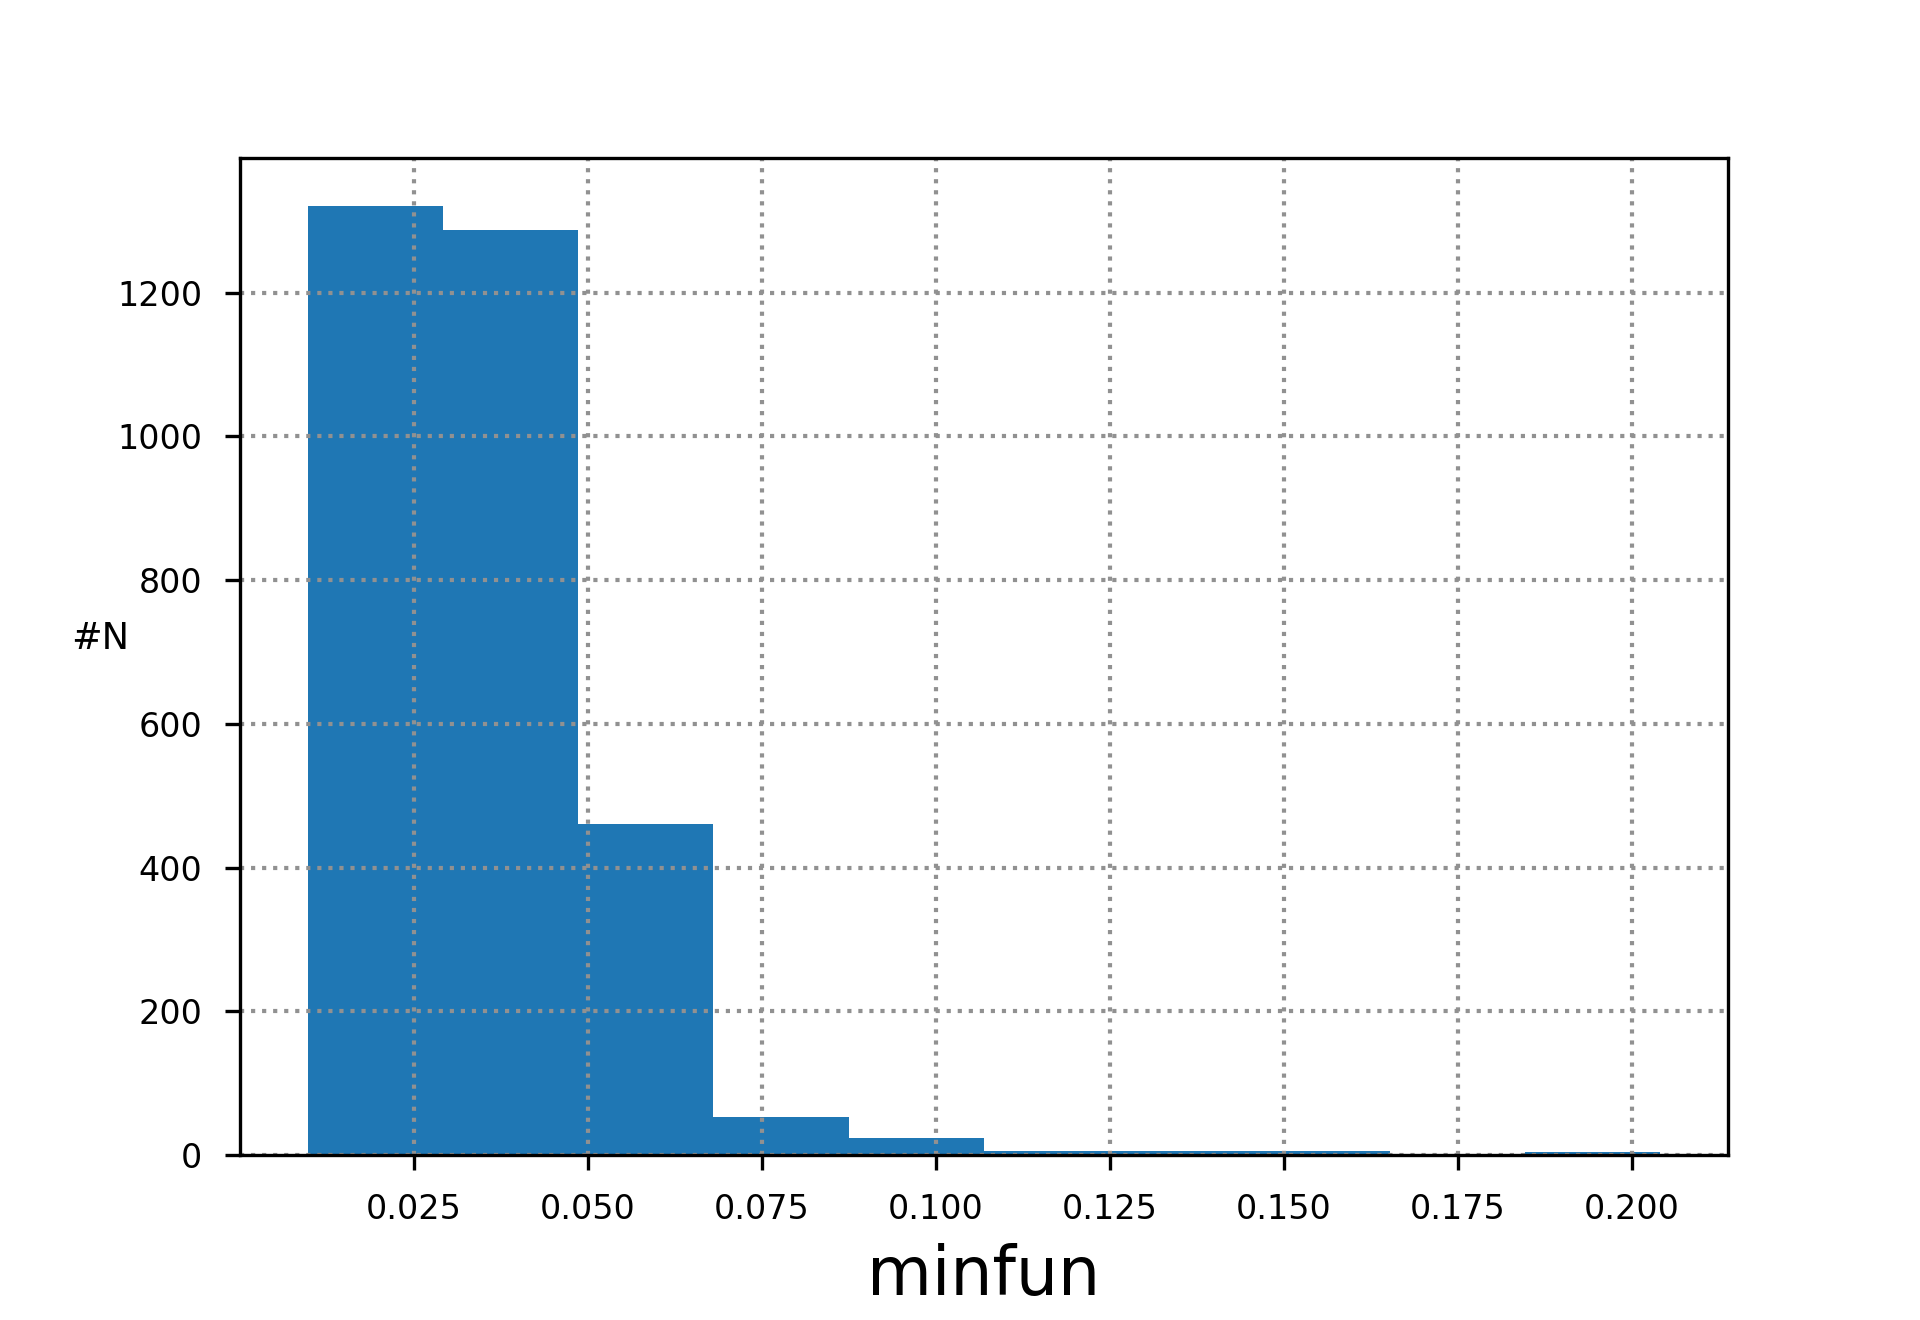
\includegraphics[width=.8\linewidth]{img1/data_histminfun.png}
                \caption{Min fun}
            \end{subfigure}
            \begin{subfigure}{.5\textwidth}
                \centering
                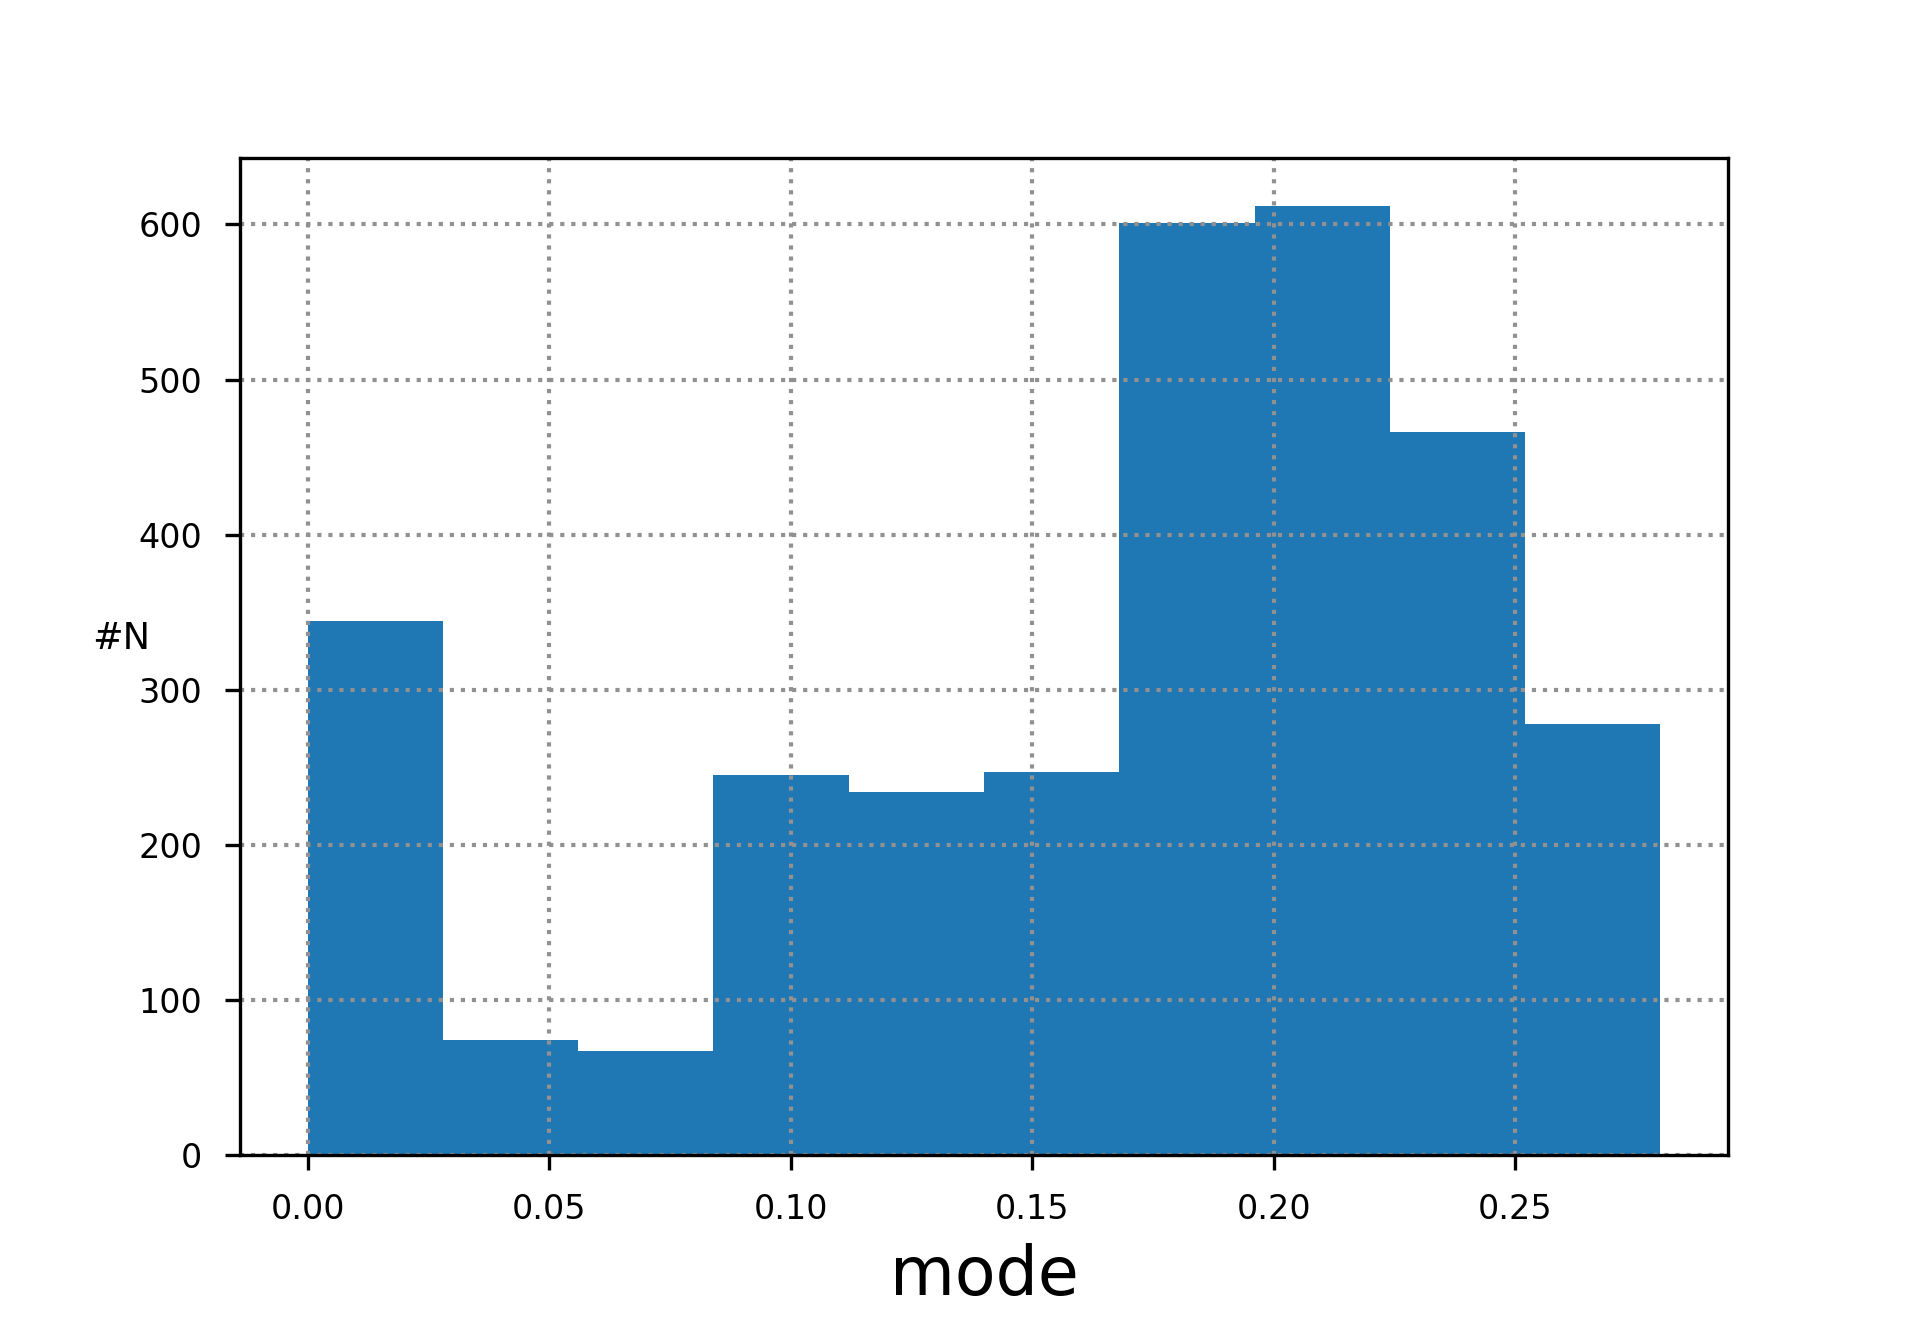
\includegraphics[width=.8\linewidth]{img1/data_histmode.png}
                \caption{Mode}
            \end{subfigure}
            \begin{subfigure}{.5\textwidth}
                \centering
                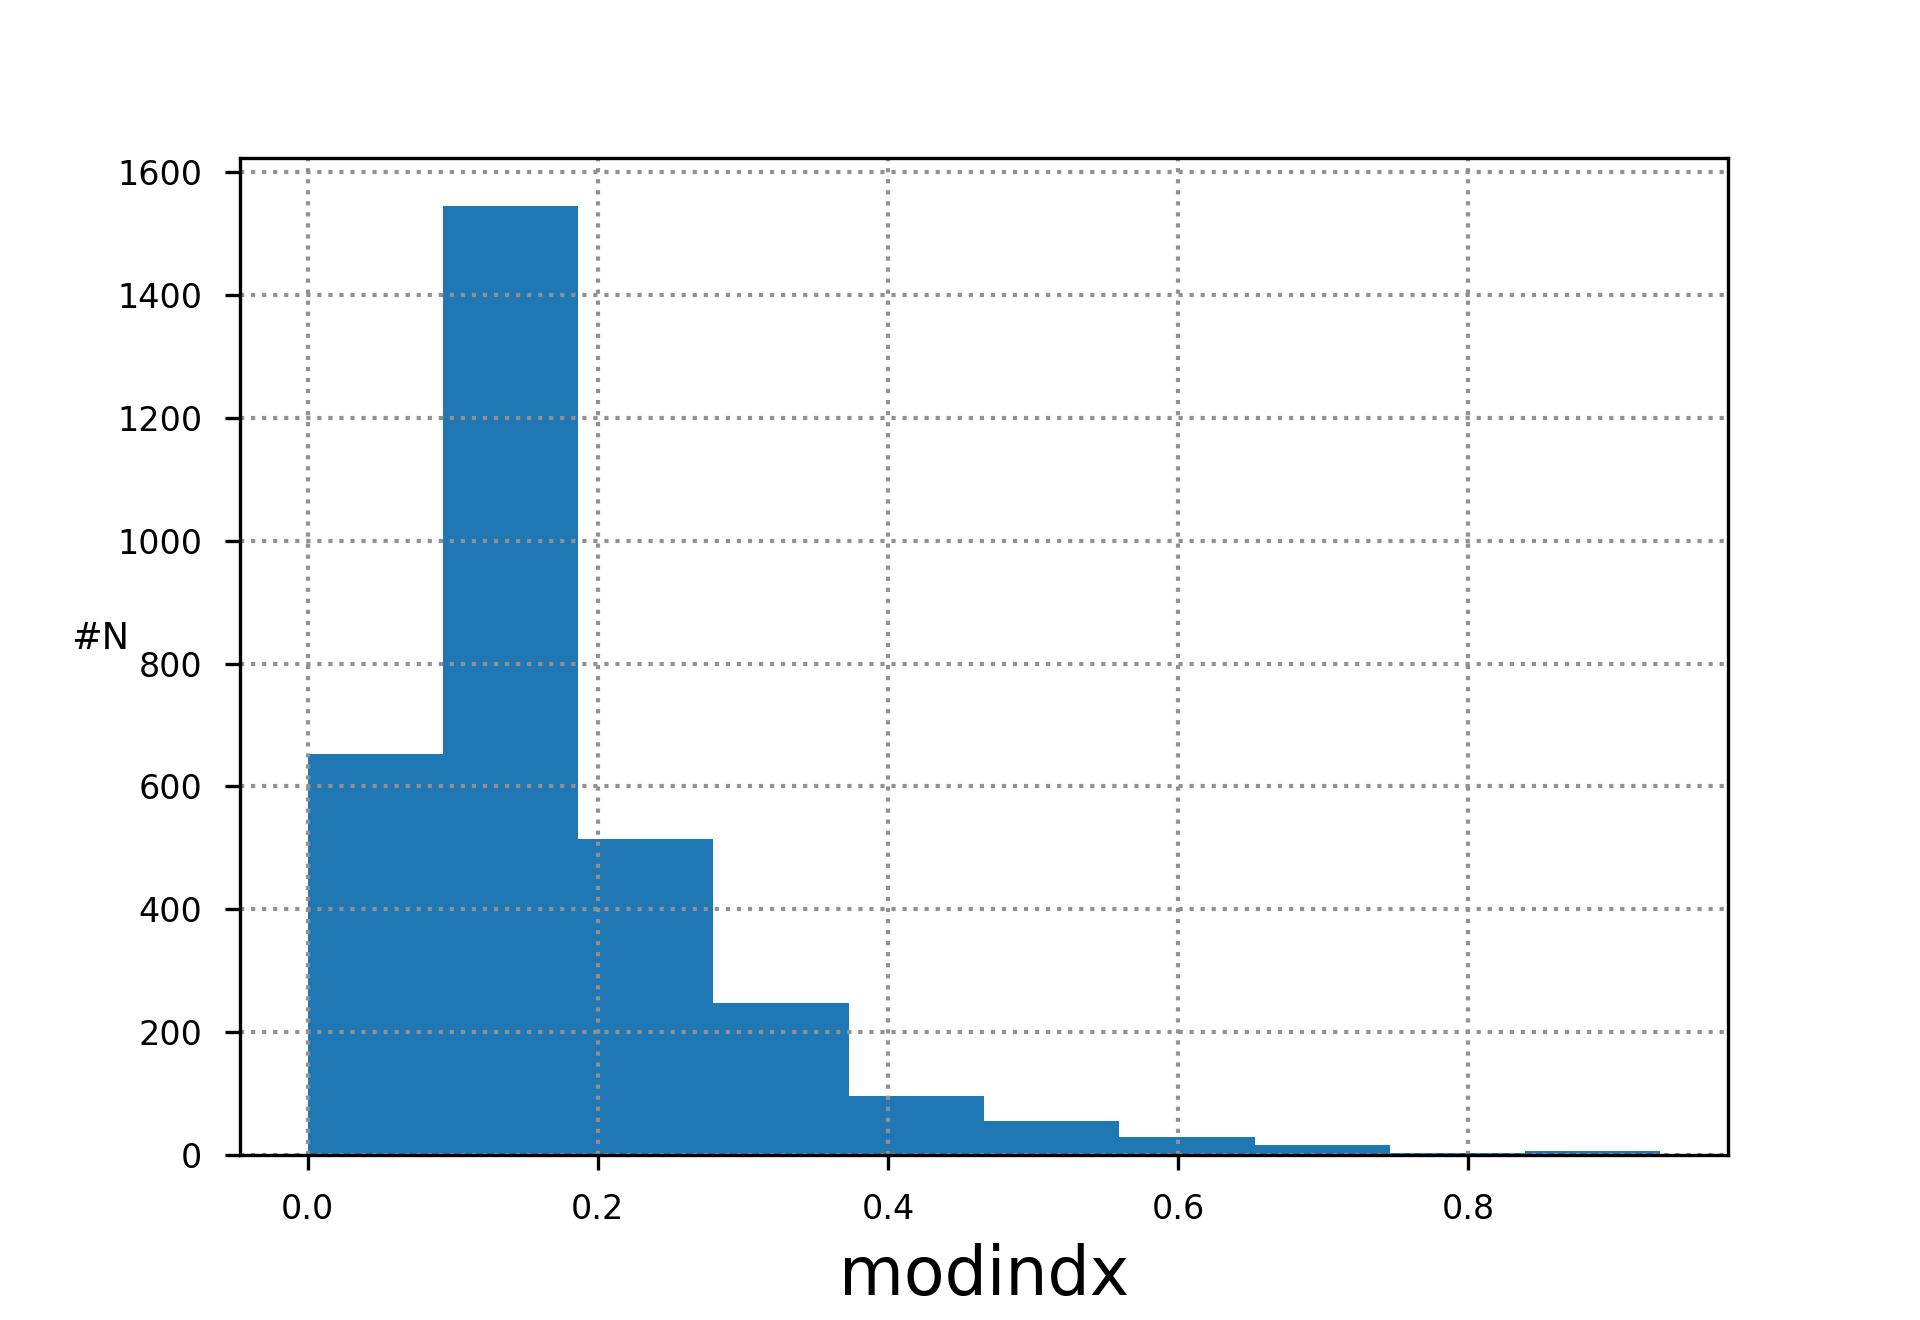
\includegraphics[width=.8\linewidth]{img1/data_histmodindx.png}
                \caption{modindx}
            \end{subfigure}
            \begin{subfigure}{.5\textwidth}
                \centering
                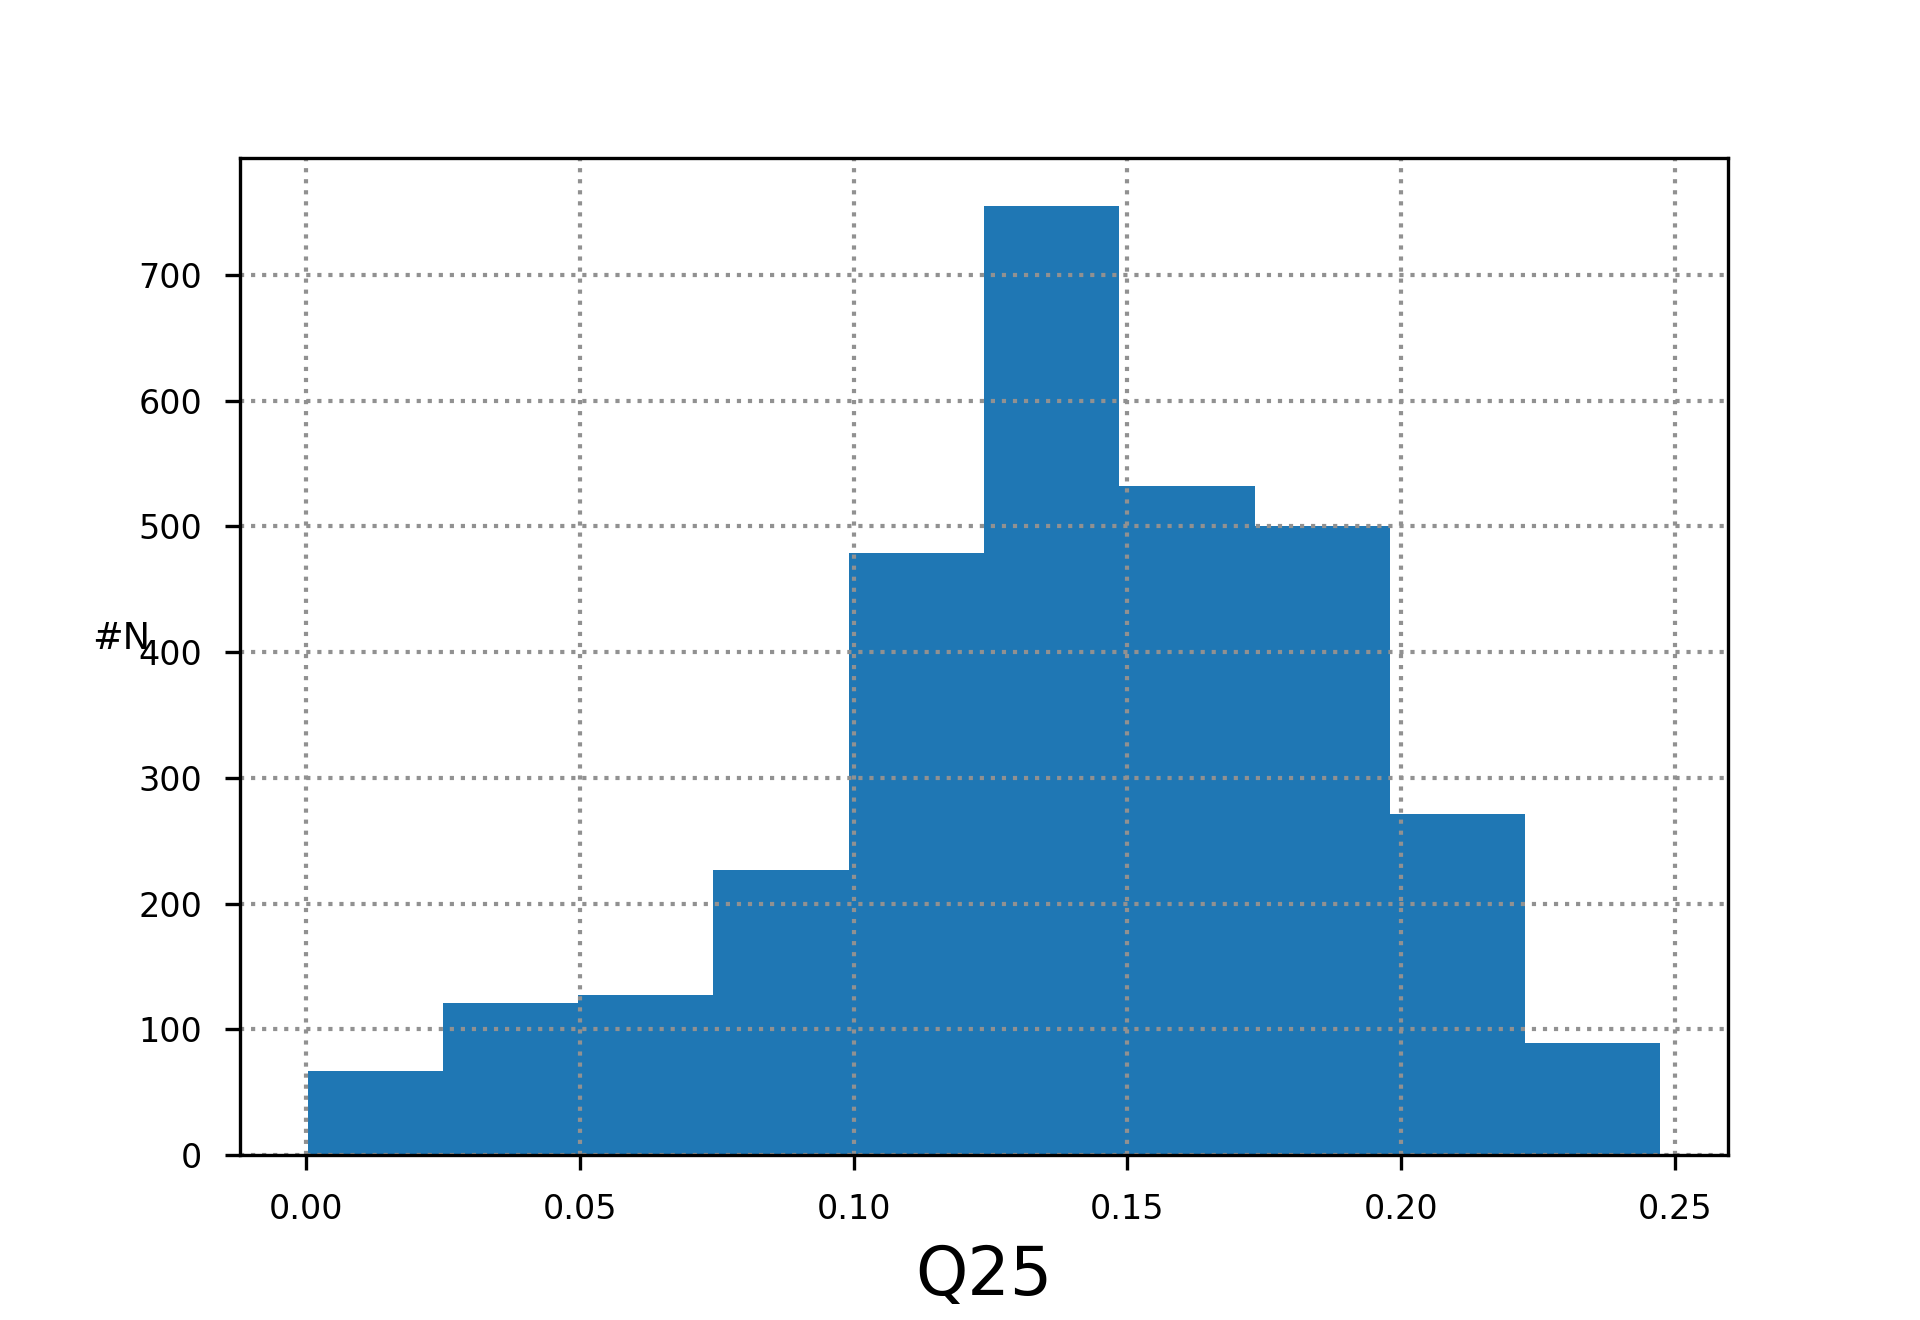
\includegraphics[width=.8\linewidth]{img1/data_histQ25.png}
                \caption{Q25}
            \end{subfigure}
            \begin{subfigure}{.5\textwidth}
                \centering
                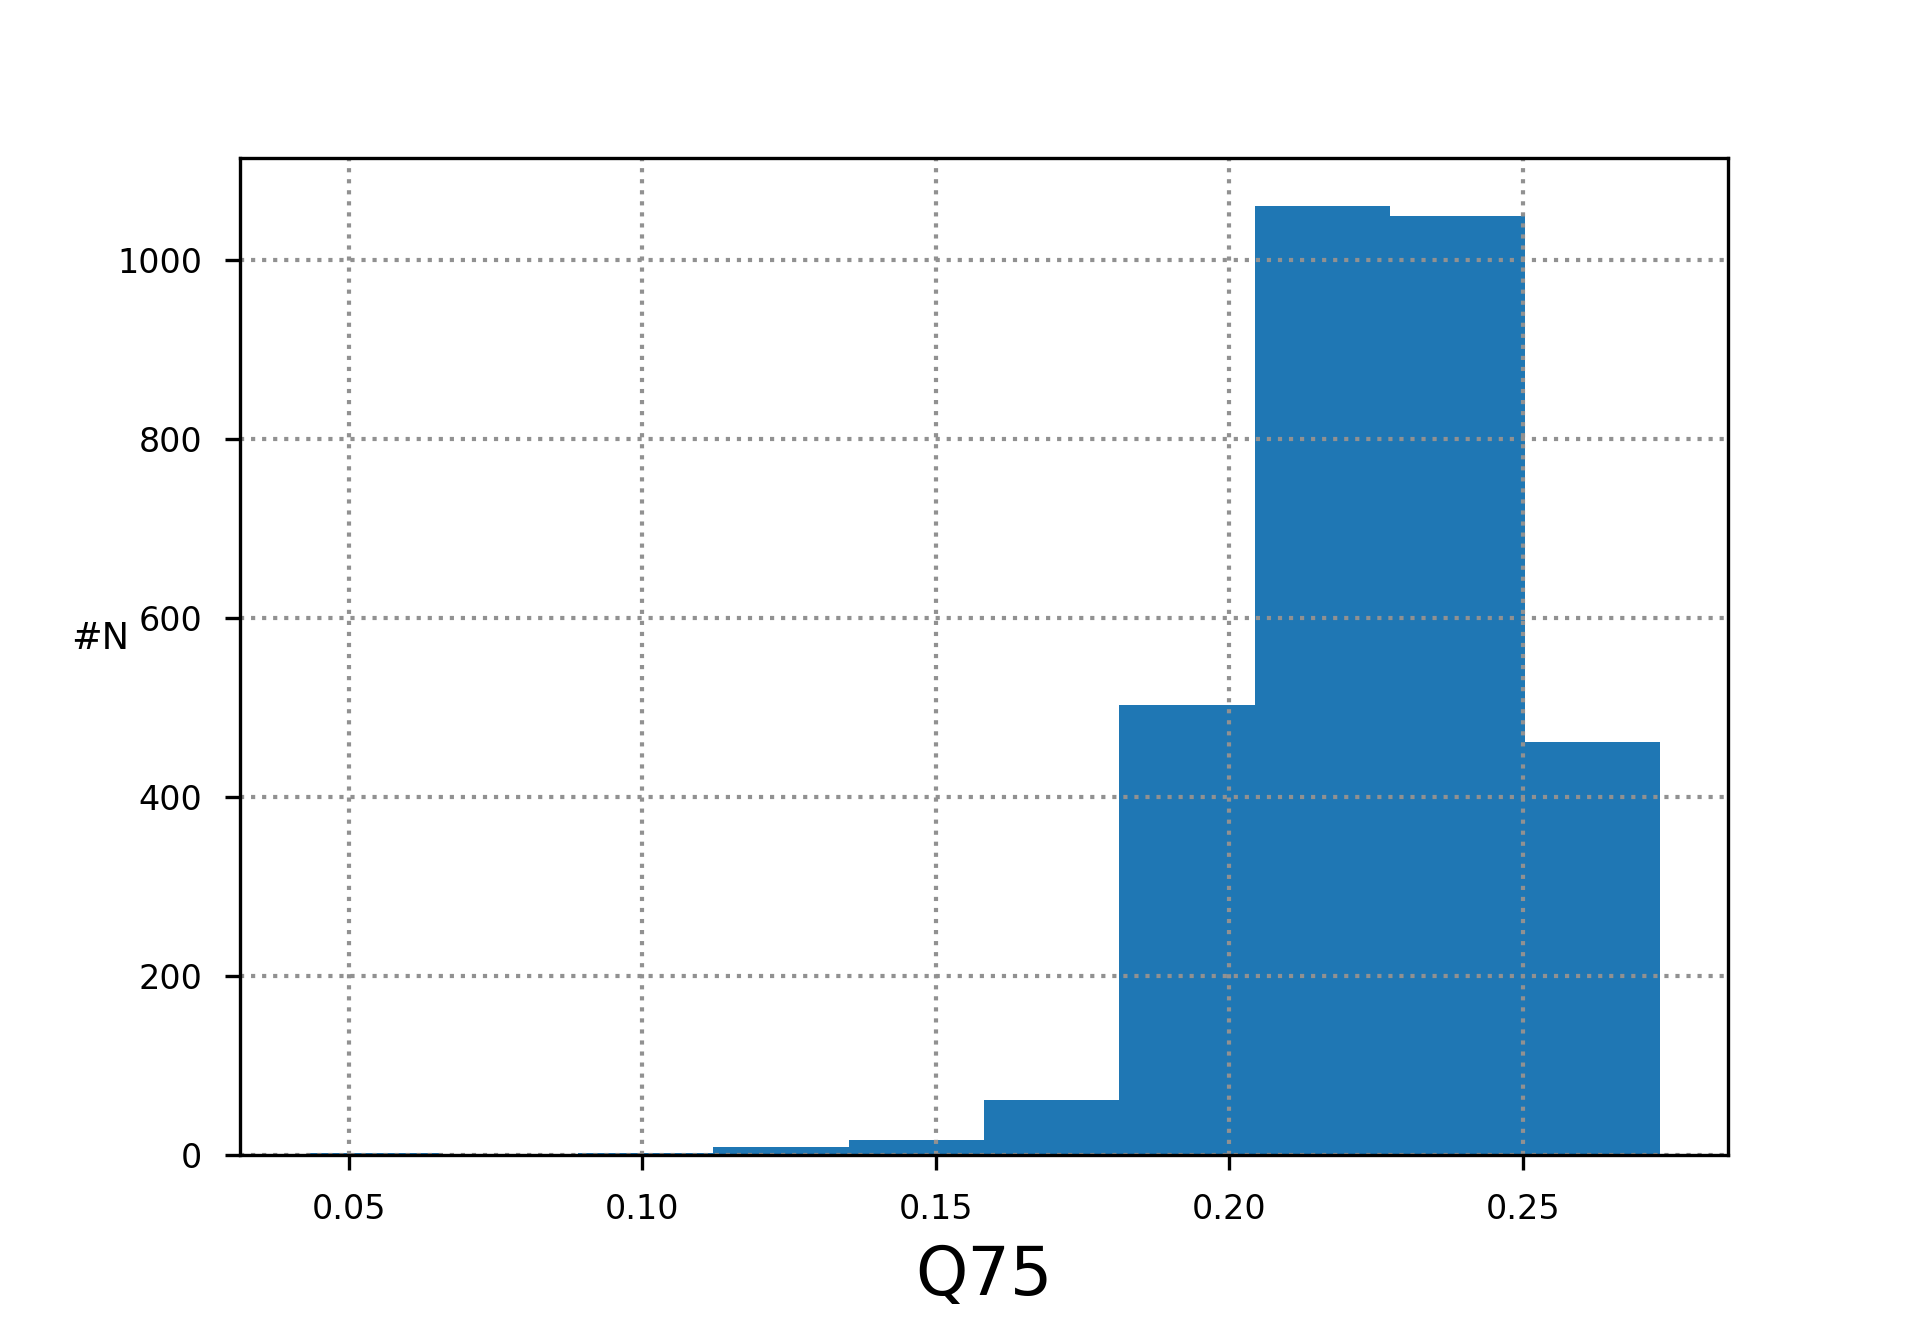
\includegraphics[width=.8\linewidth]{img1/data_histQ75.png}
                \caption{Q75}
            \end{subfigure}
            \begin{subfigure}{.5\textwidth}
                \centering
                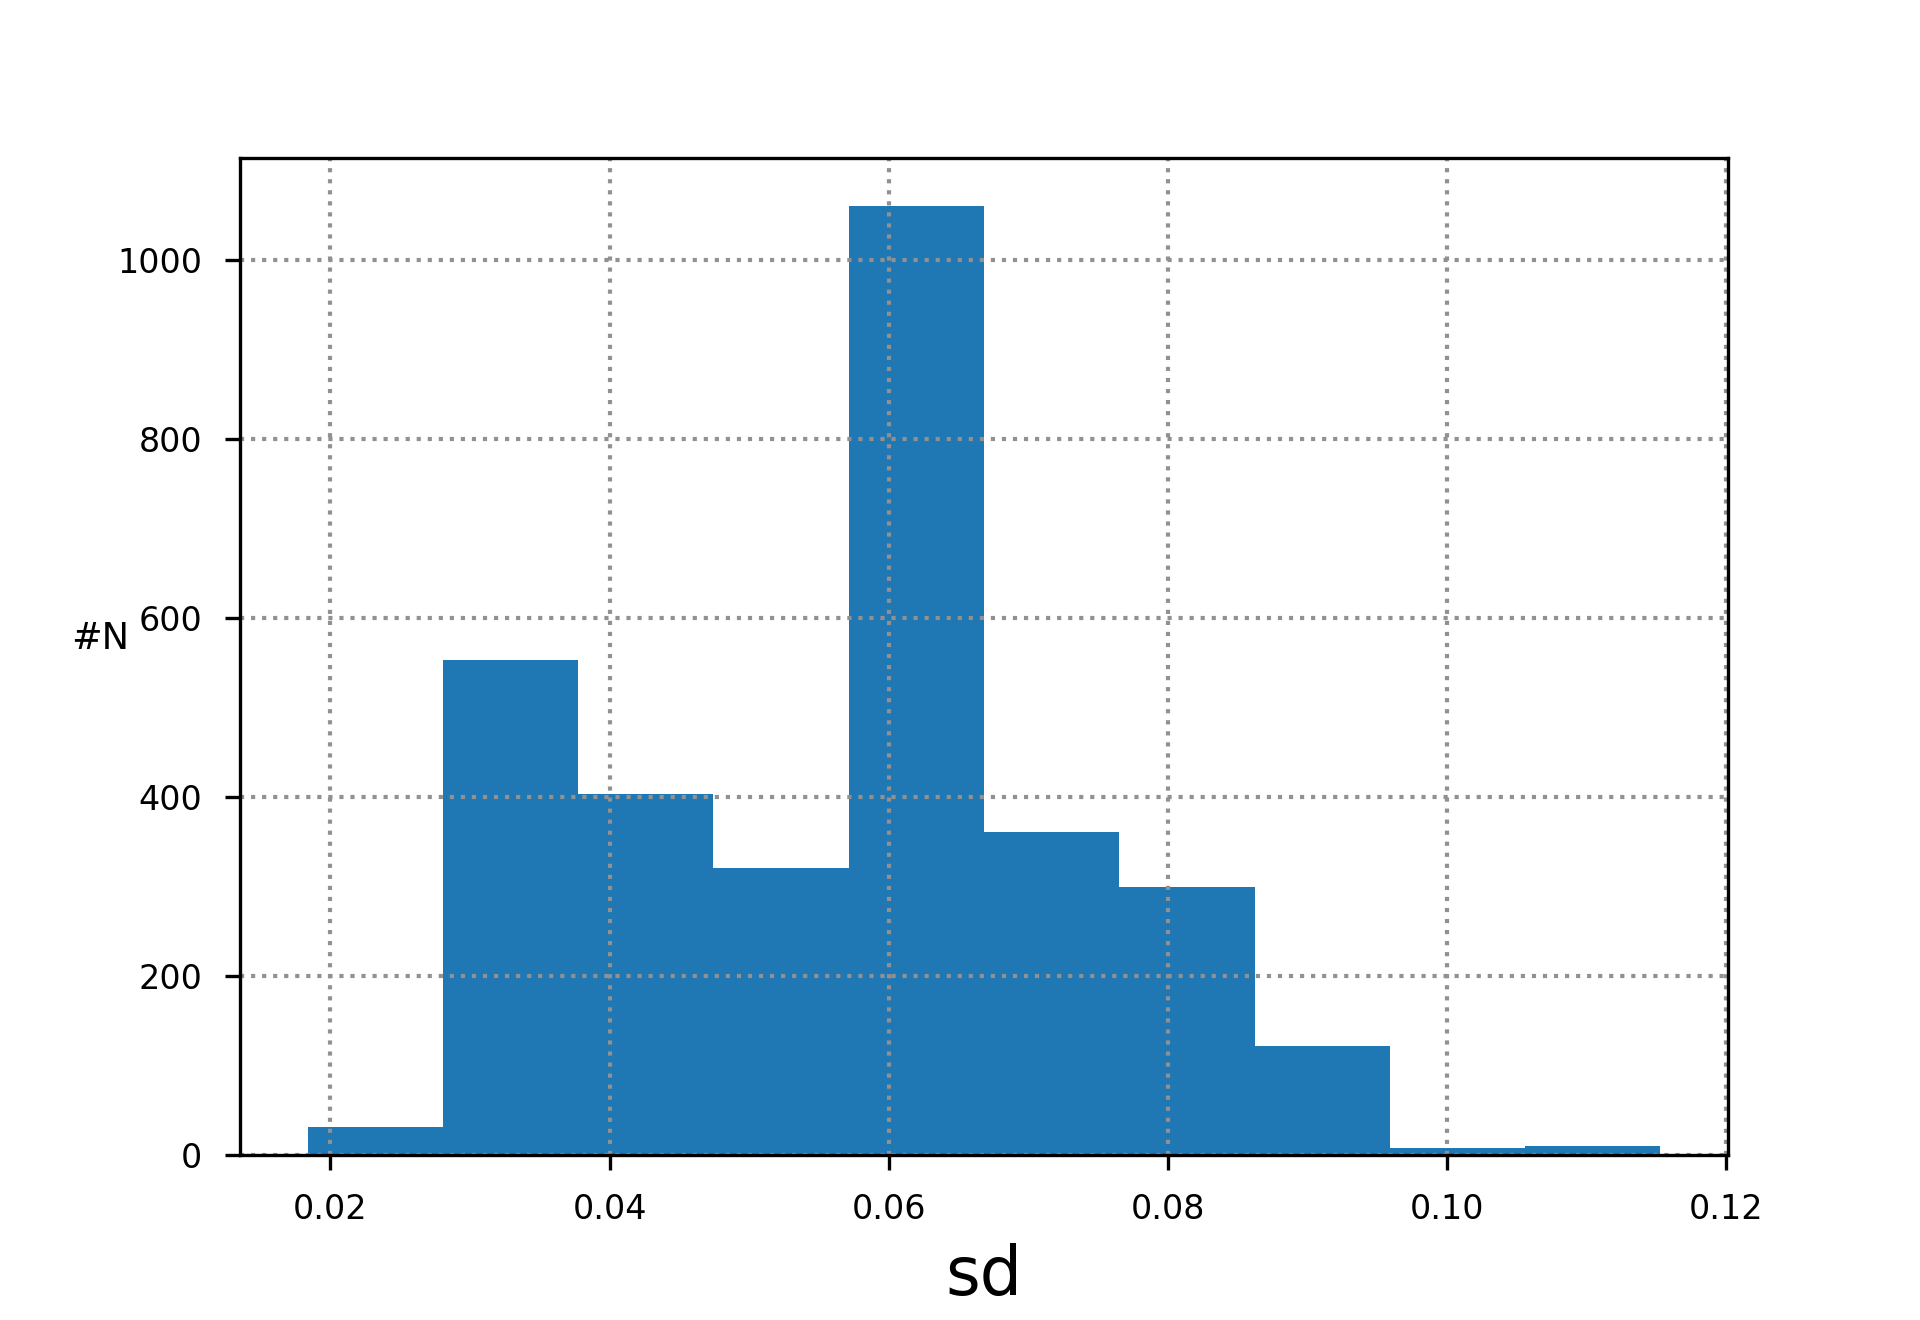
\includegraphics[width=.8\linewidth]{img1/data_histsd.png}
                \caption{sd}
            \end{subfigure}
            \begin{subfigure}{.5\textwidth}
                \centering
                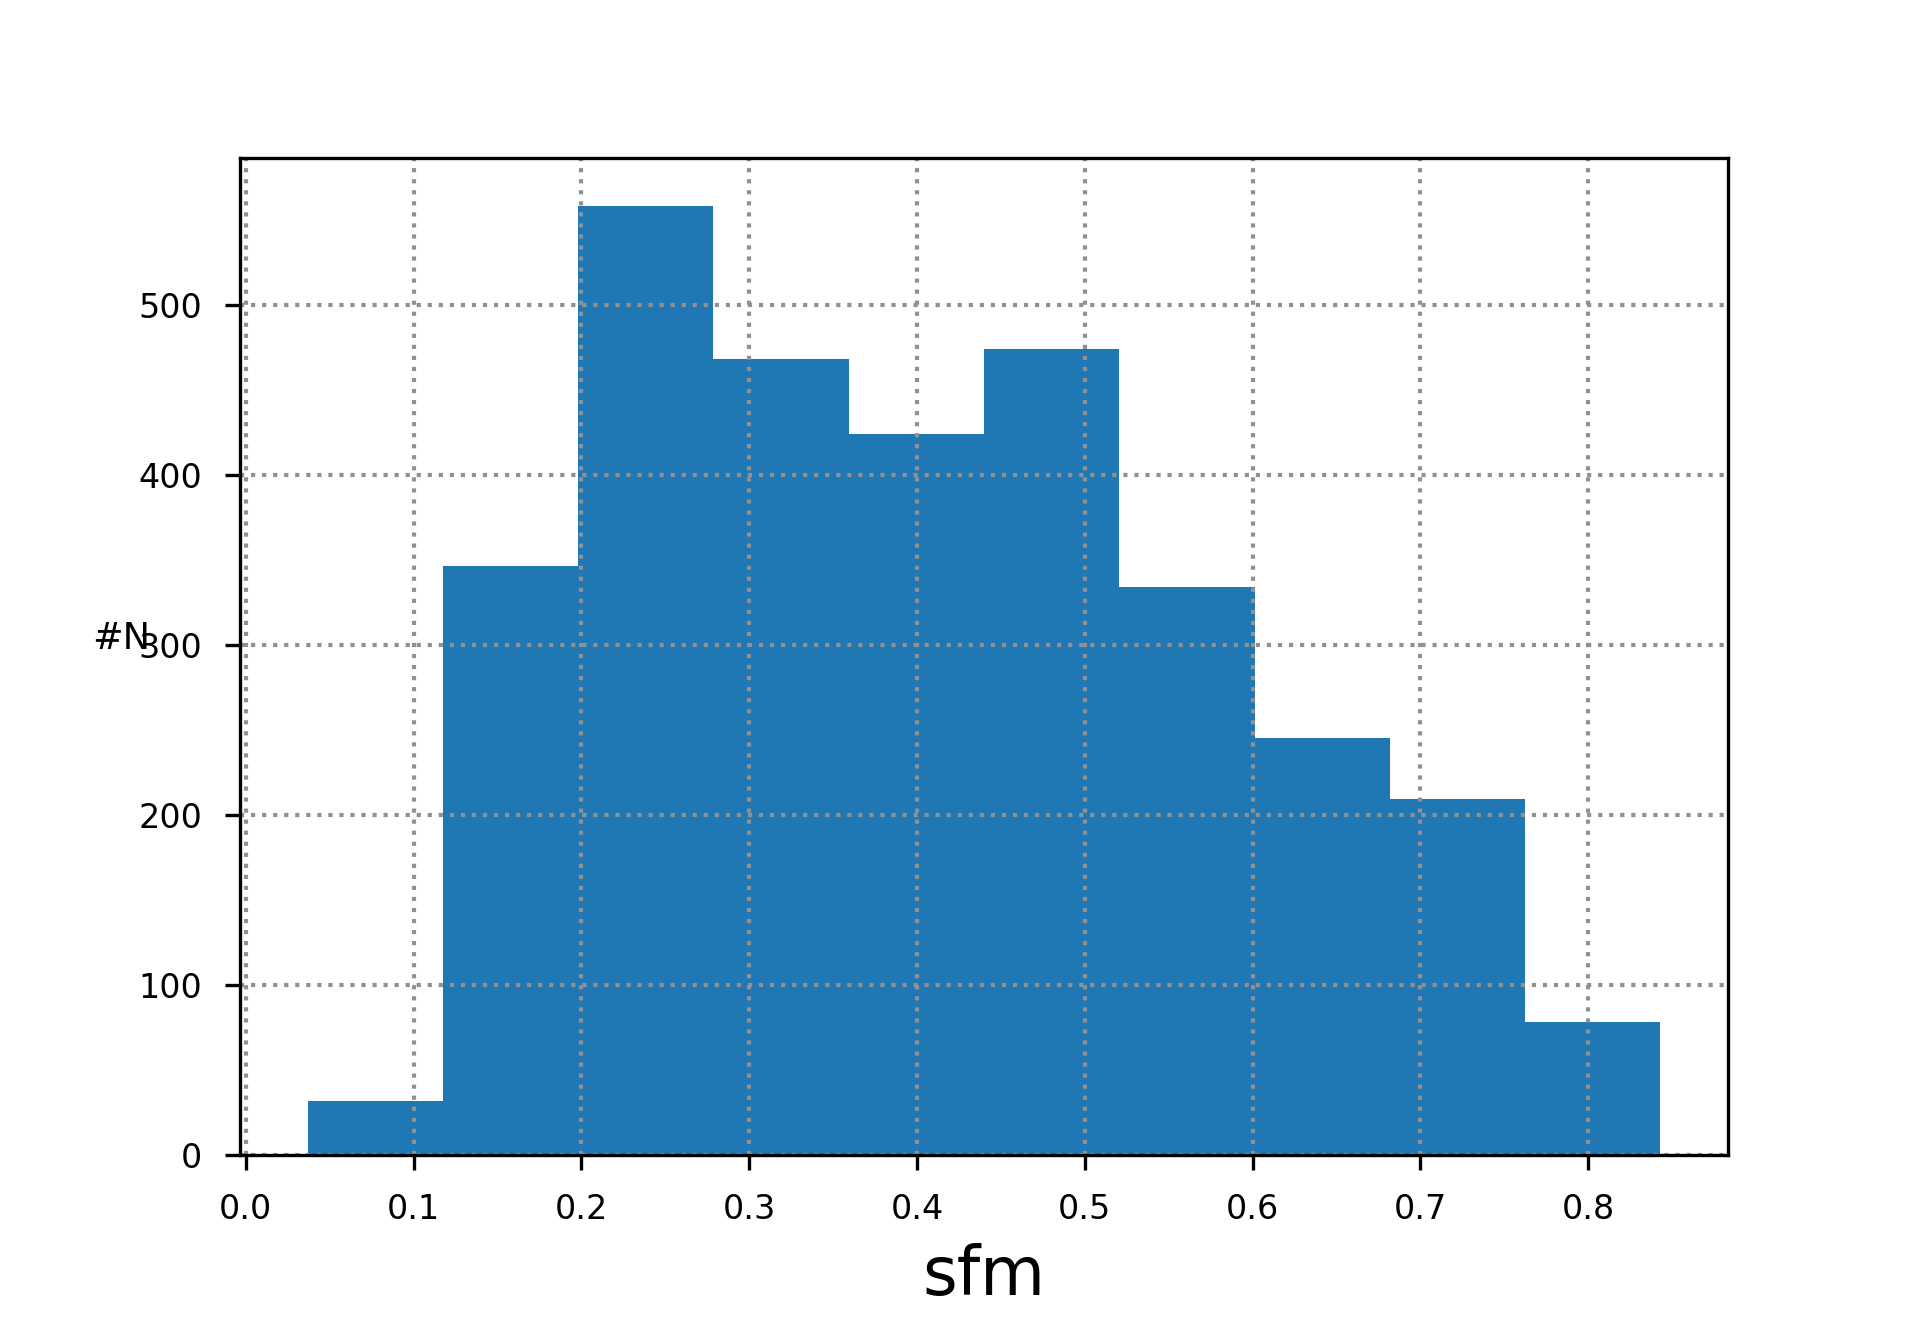
\includegraphics[width=.8\linewidth]{img1/data_histsfm.png}
                \caption{sfm}
            \end{subfigure}
        \caption{Classificação binária: Histograma dos atributos (2)}
        \label{fig:a_hist_2}
        \end{figure}
        \begin{figure}[H]
            \begin{subfigure}{.5\textwidth}
                \centering
                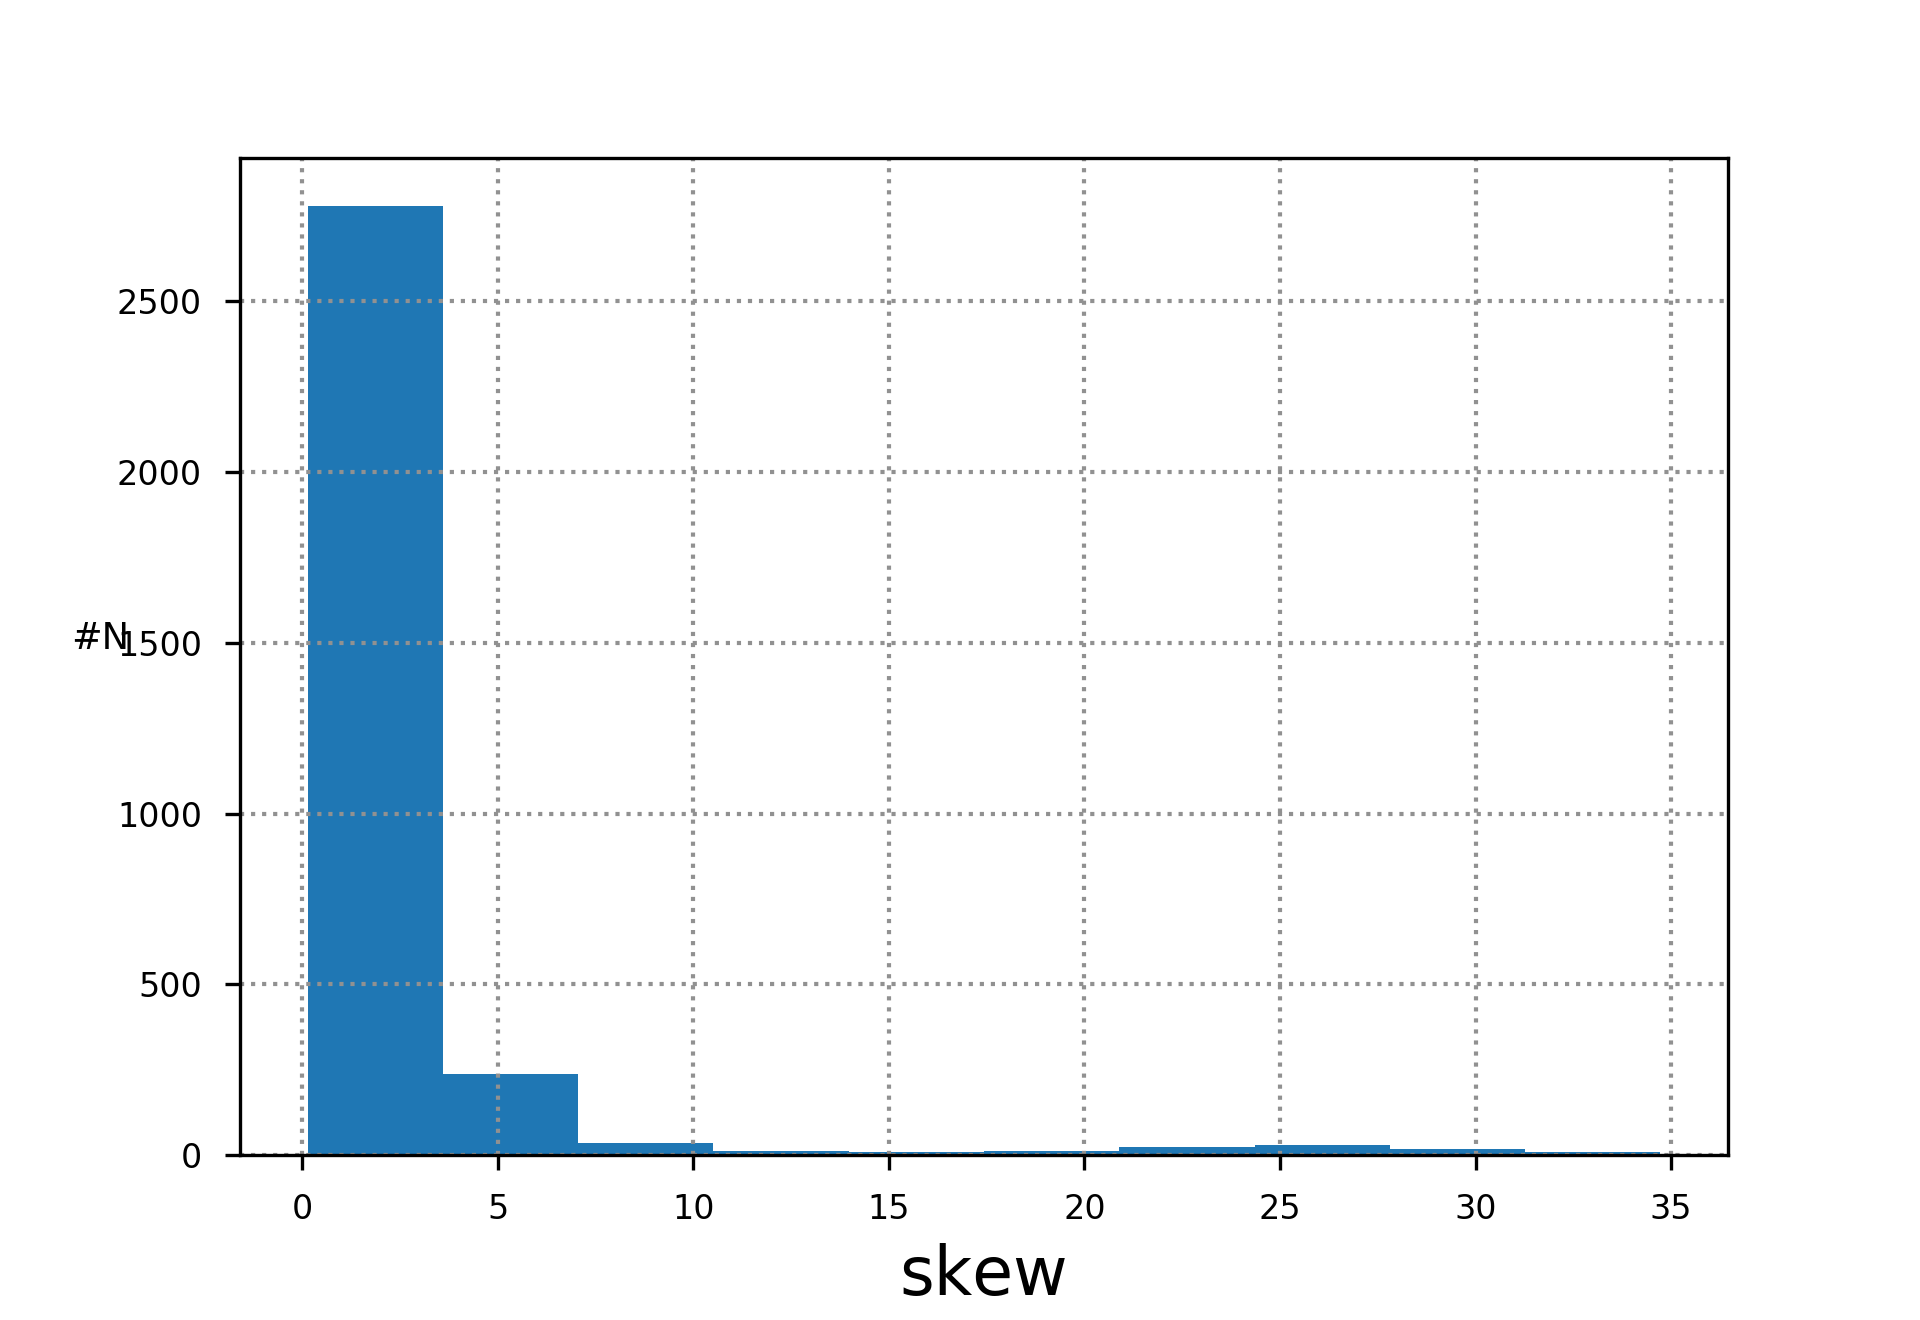
\includegraphics[width=.8\linewidth]{img1/data_histskew.png}
                \caption{skew}
            \end{subfigure}
            \begin{subfigure}{.5\textwidth}
                \centering
                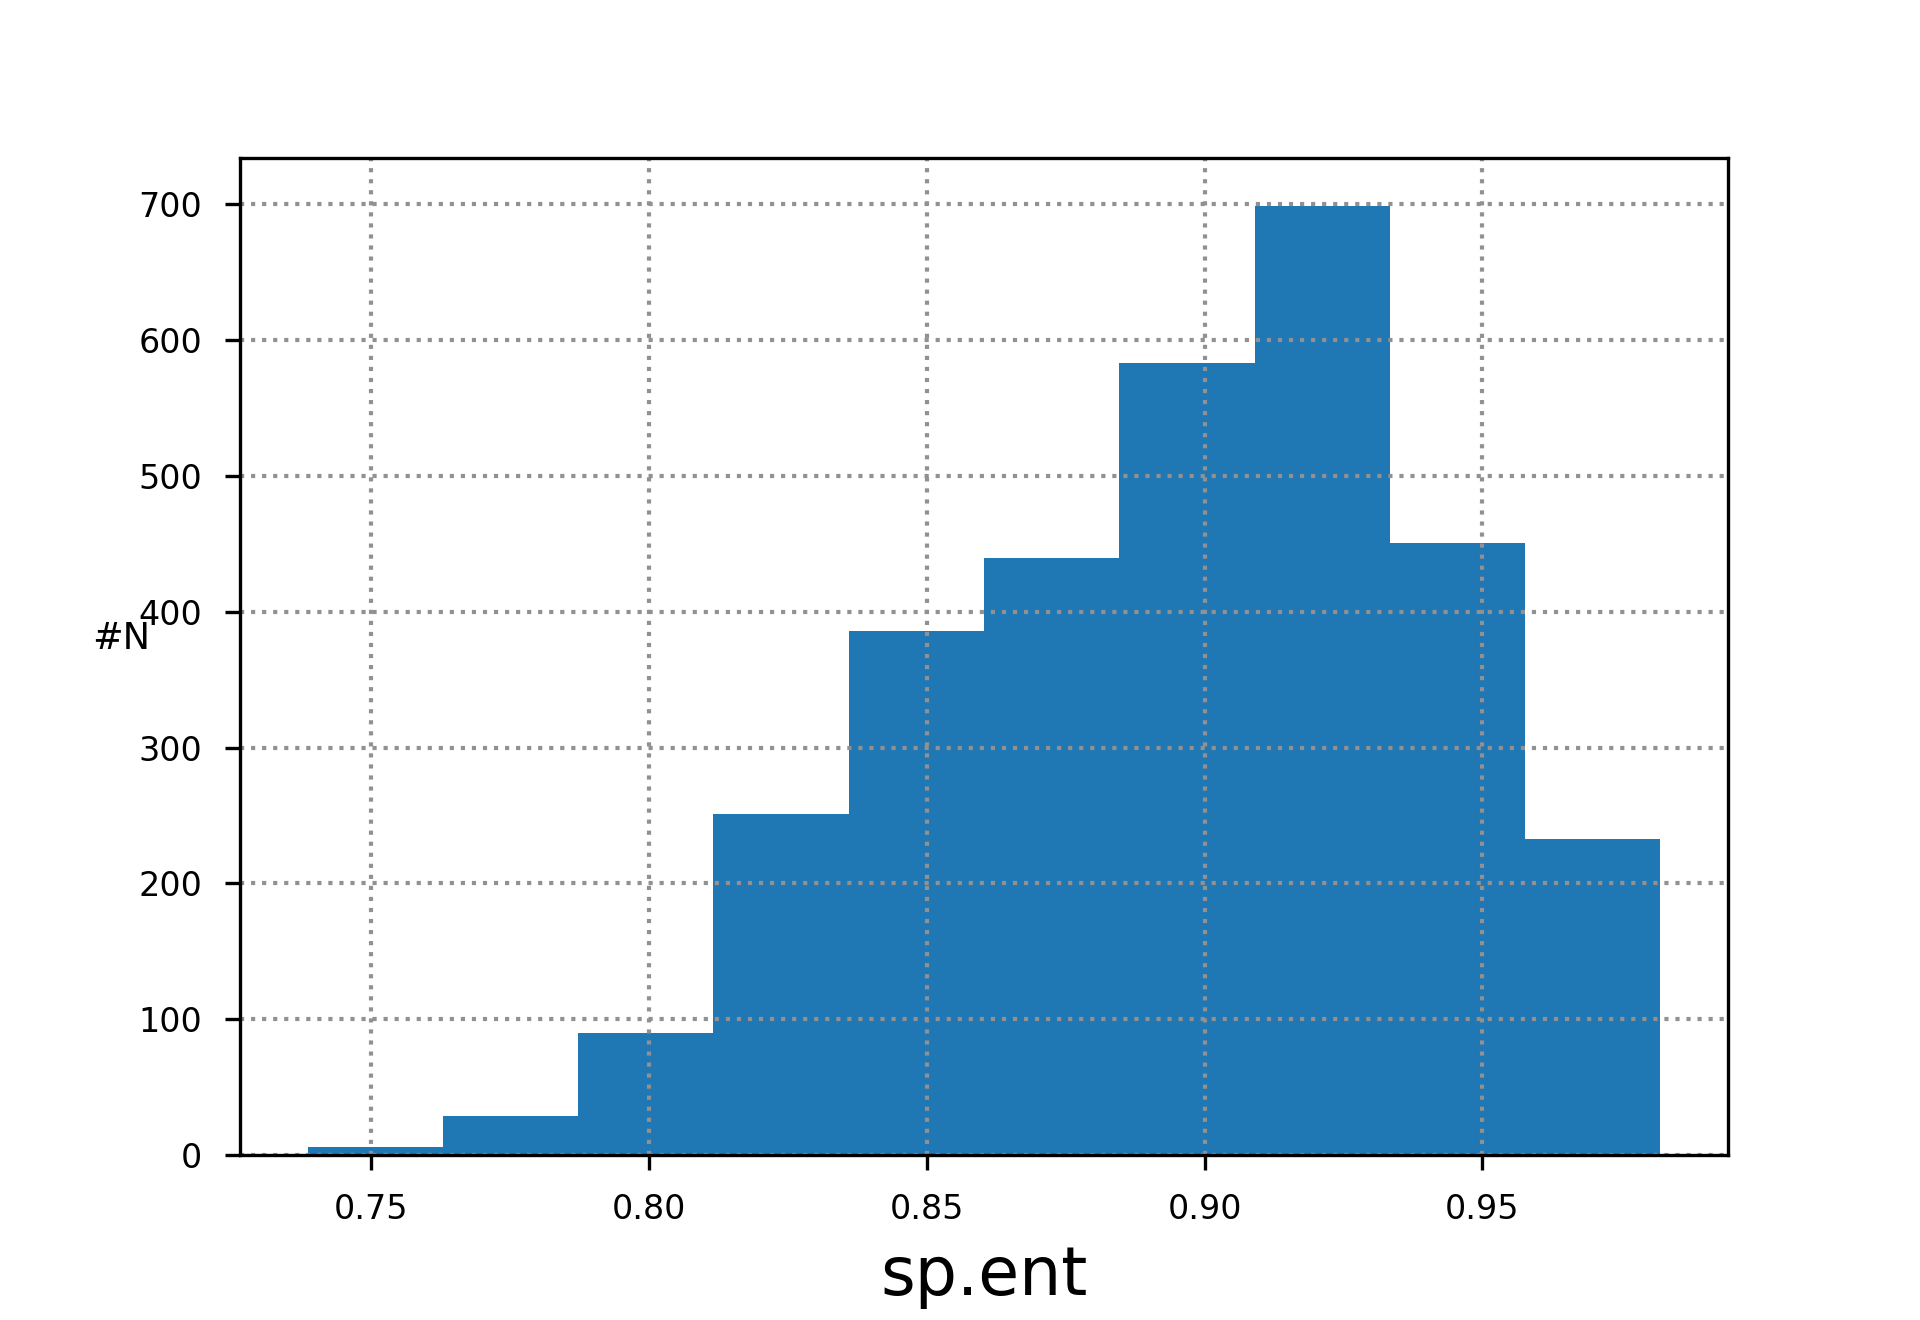
\includegraphics[width=.8\linewidth]{img1/data_histsp_ent.png}
                \caption{histsp.ent}
            \end{subfigure}
            \begin{subfigure}{.5\textwidth}
                \centering
                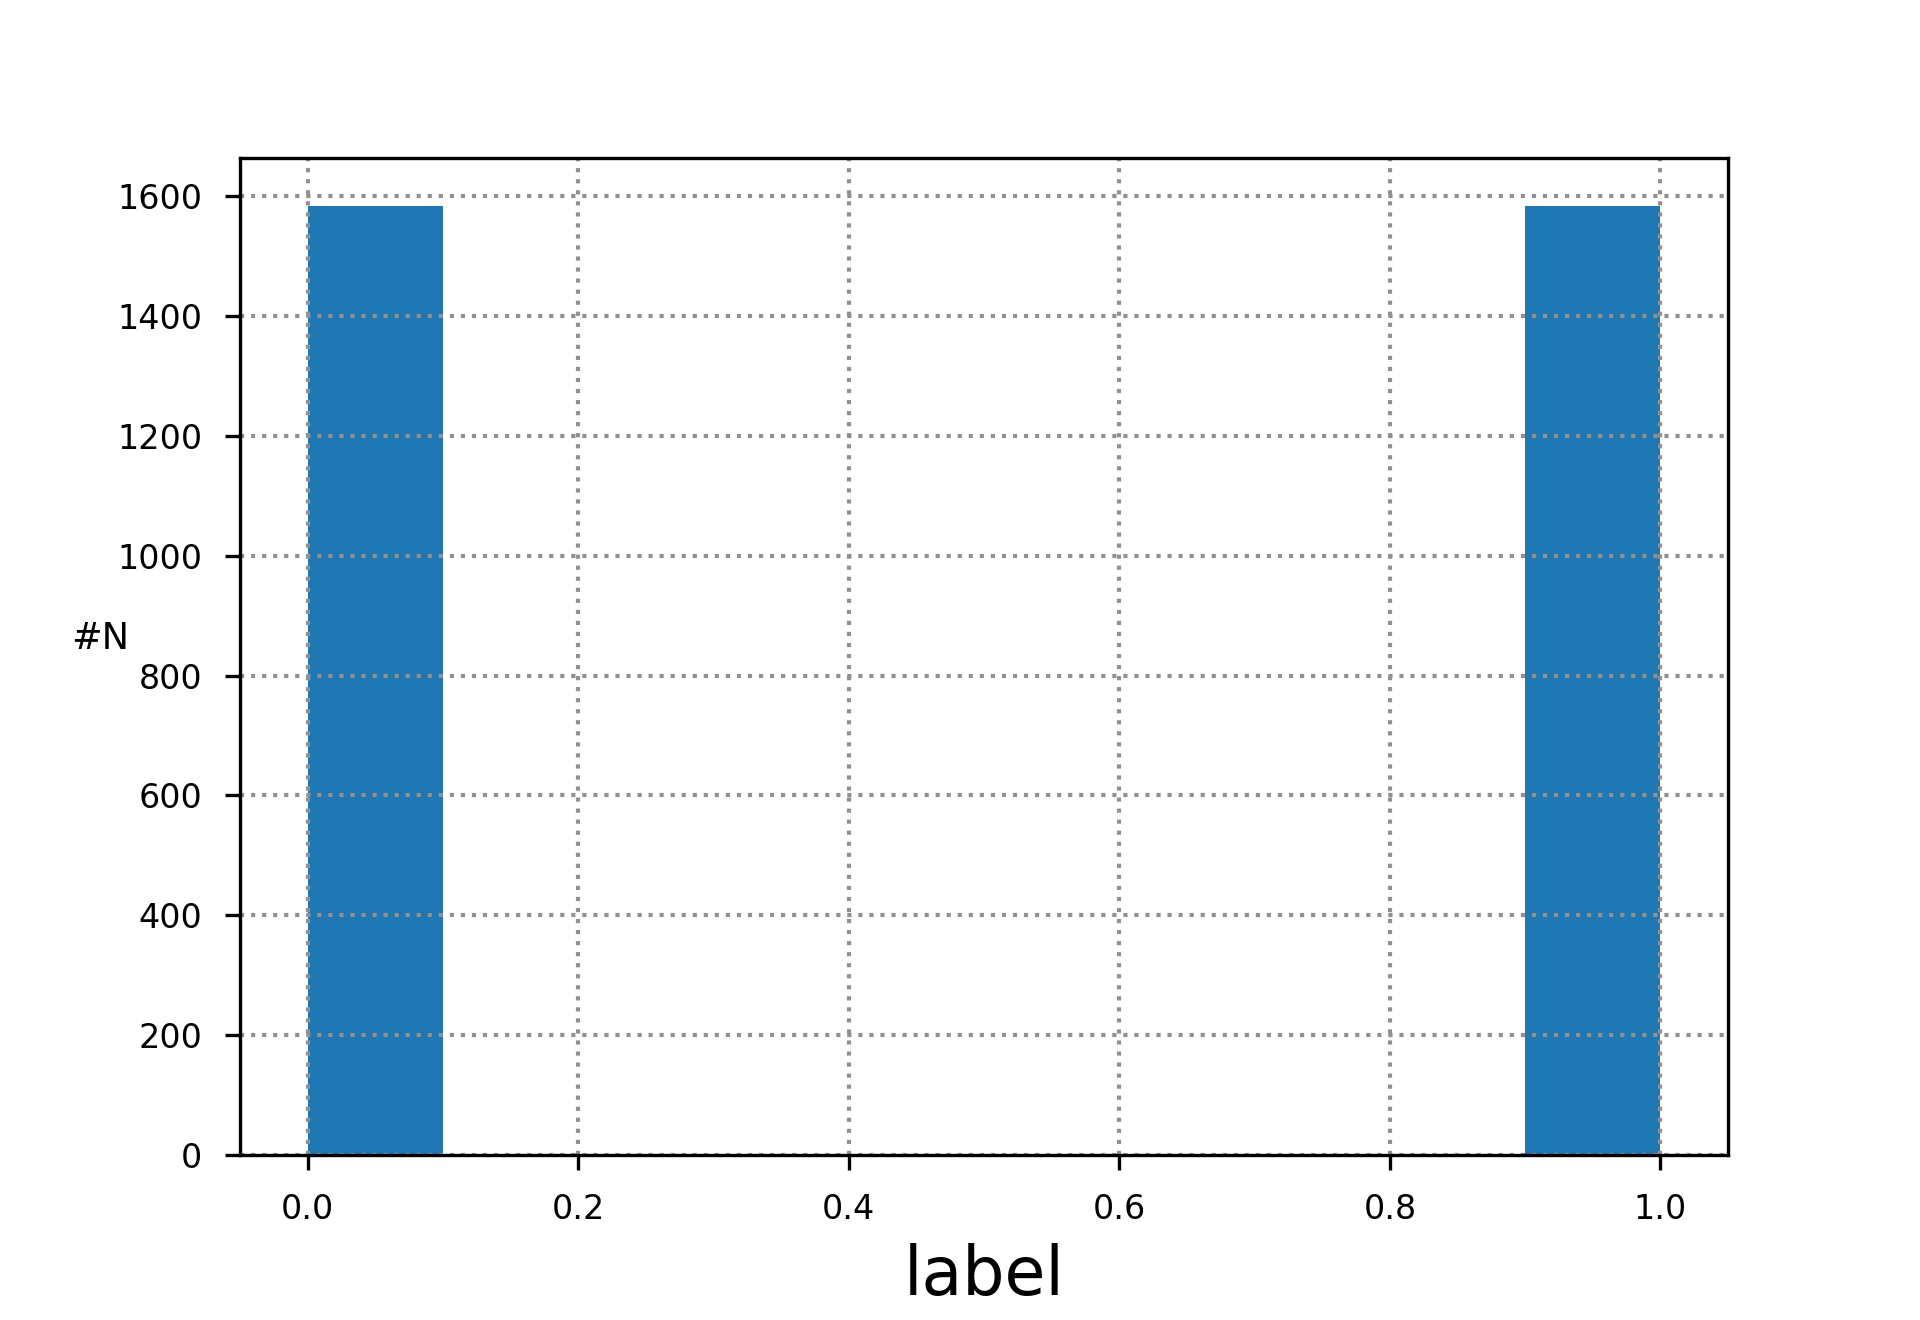
\includegraphics[width=.8\linewidth]{img1/data_histlabel.png}
                \caption{label}
            \end{subfigure}
        \caption{Classificação binária: Histograma dos atributos (3)}
        \label{fig:a_hist_3}
        \end{figure}

        \begin{figure}[H]
            \centering
            \includegraphics[width=.8\linewidth]{img1/data_corr.png}
            \caption{Classificação binária: Mapa de calor da correlaçao dos atributos}
            \label{fig:a_corr_heat}
        \end{figure}
        \begin{figure}[H]
            \centering
            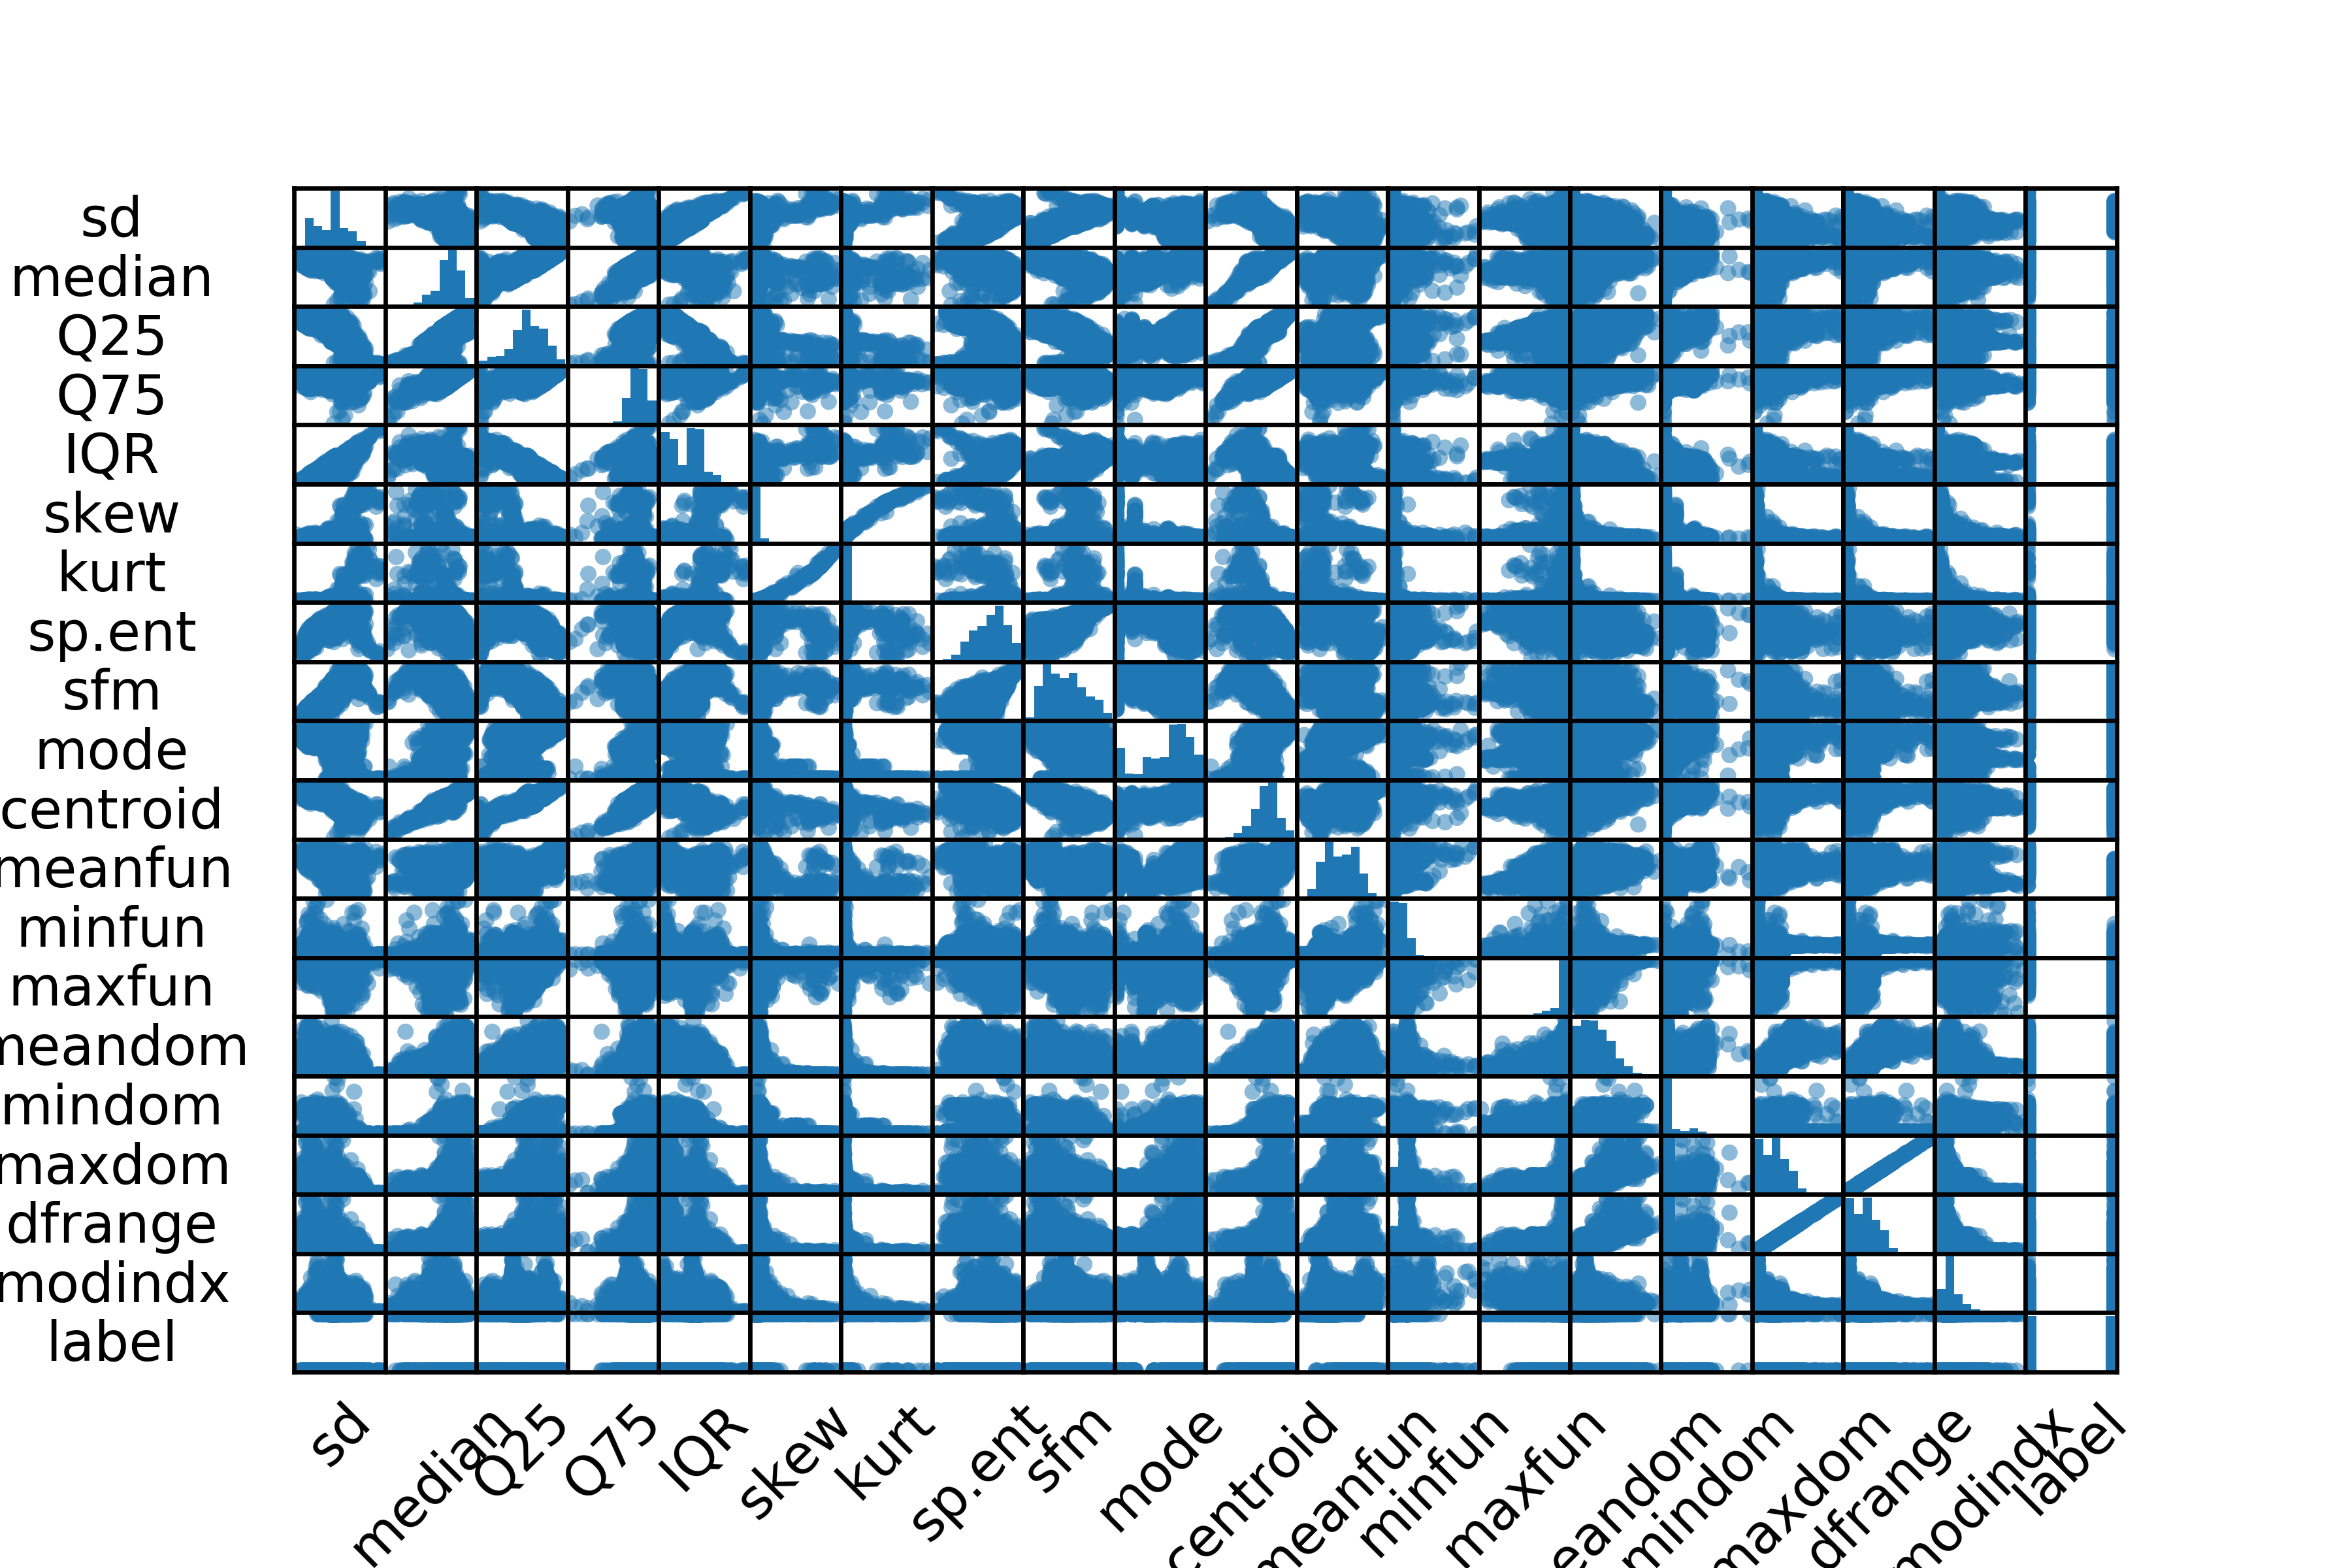
\includegraphics[width=\textwidth]{img1/data_corr_scatter.png}
            \caption{Classificação binária: Correlação dos atributos em gráfico de dispersão }
            \label{fig:a_corr_scatter}
        \end{figure}
    \subsection[]{b) Curva ROC e $F_1$-medida}
        É utilizado o método \textit{Z-score} para normalização dos dados. Tal método foi escolhido
        pois favorece o progresso de algoritmos baseados no gradiente descendente, uma vez que deixa as curvas de nível
        da superfície de erro mais circulares.

        O processo de treinamento tem como critério de parada a variação da função de custo. Quando
        o decréscimo por década do custo for inferior a $10^{-8}$ é terminado o processo de treinamento.

        Parâmetros de treinamento, sendo $\eta$ a taxa de aprendizagem e $tol$ o limiar para o término do processo:
        \begin{align*}
            \eta&=10^{-2} \\
            tol&=10^{-8}
        \end{align*}
        A curva ROC é obtida consideranto o rótulo $1$ como classe positiva.
        \begin{figure}[H]
            \centering
            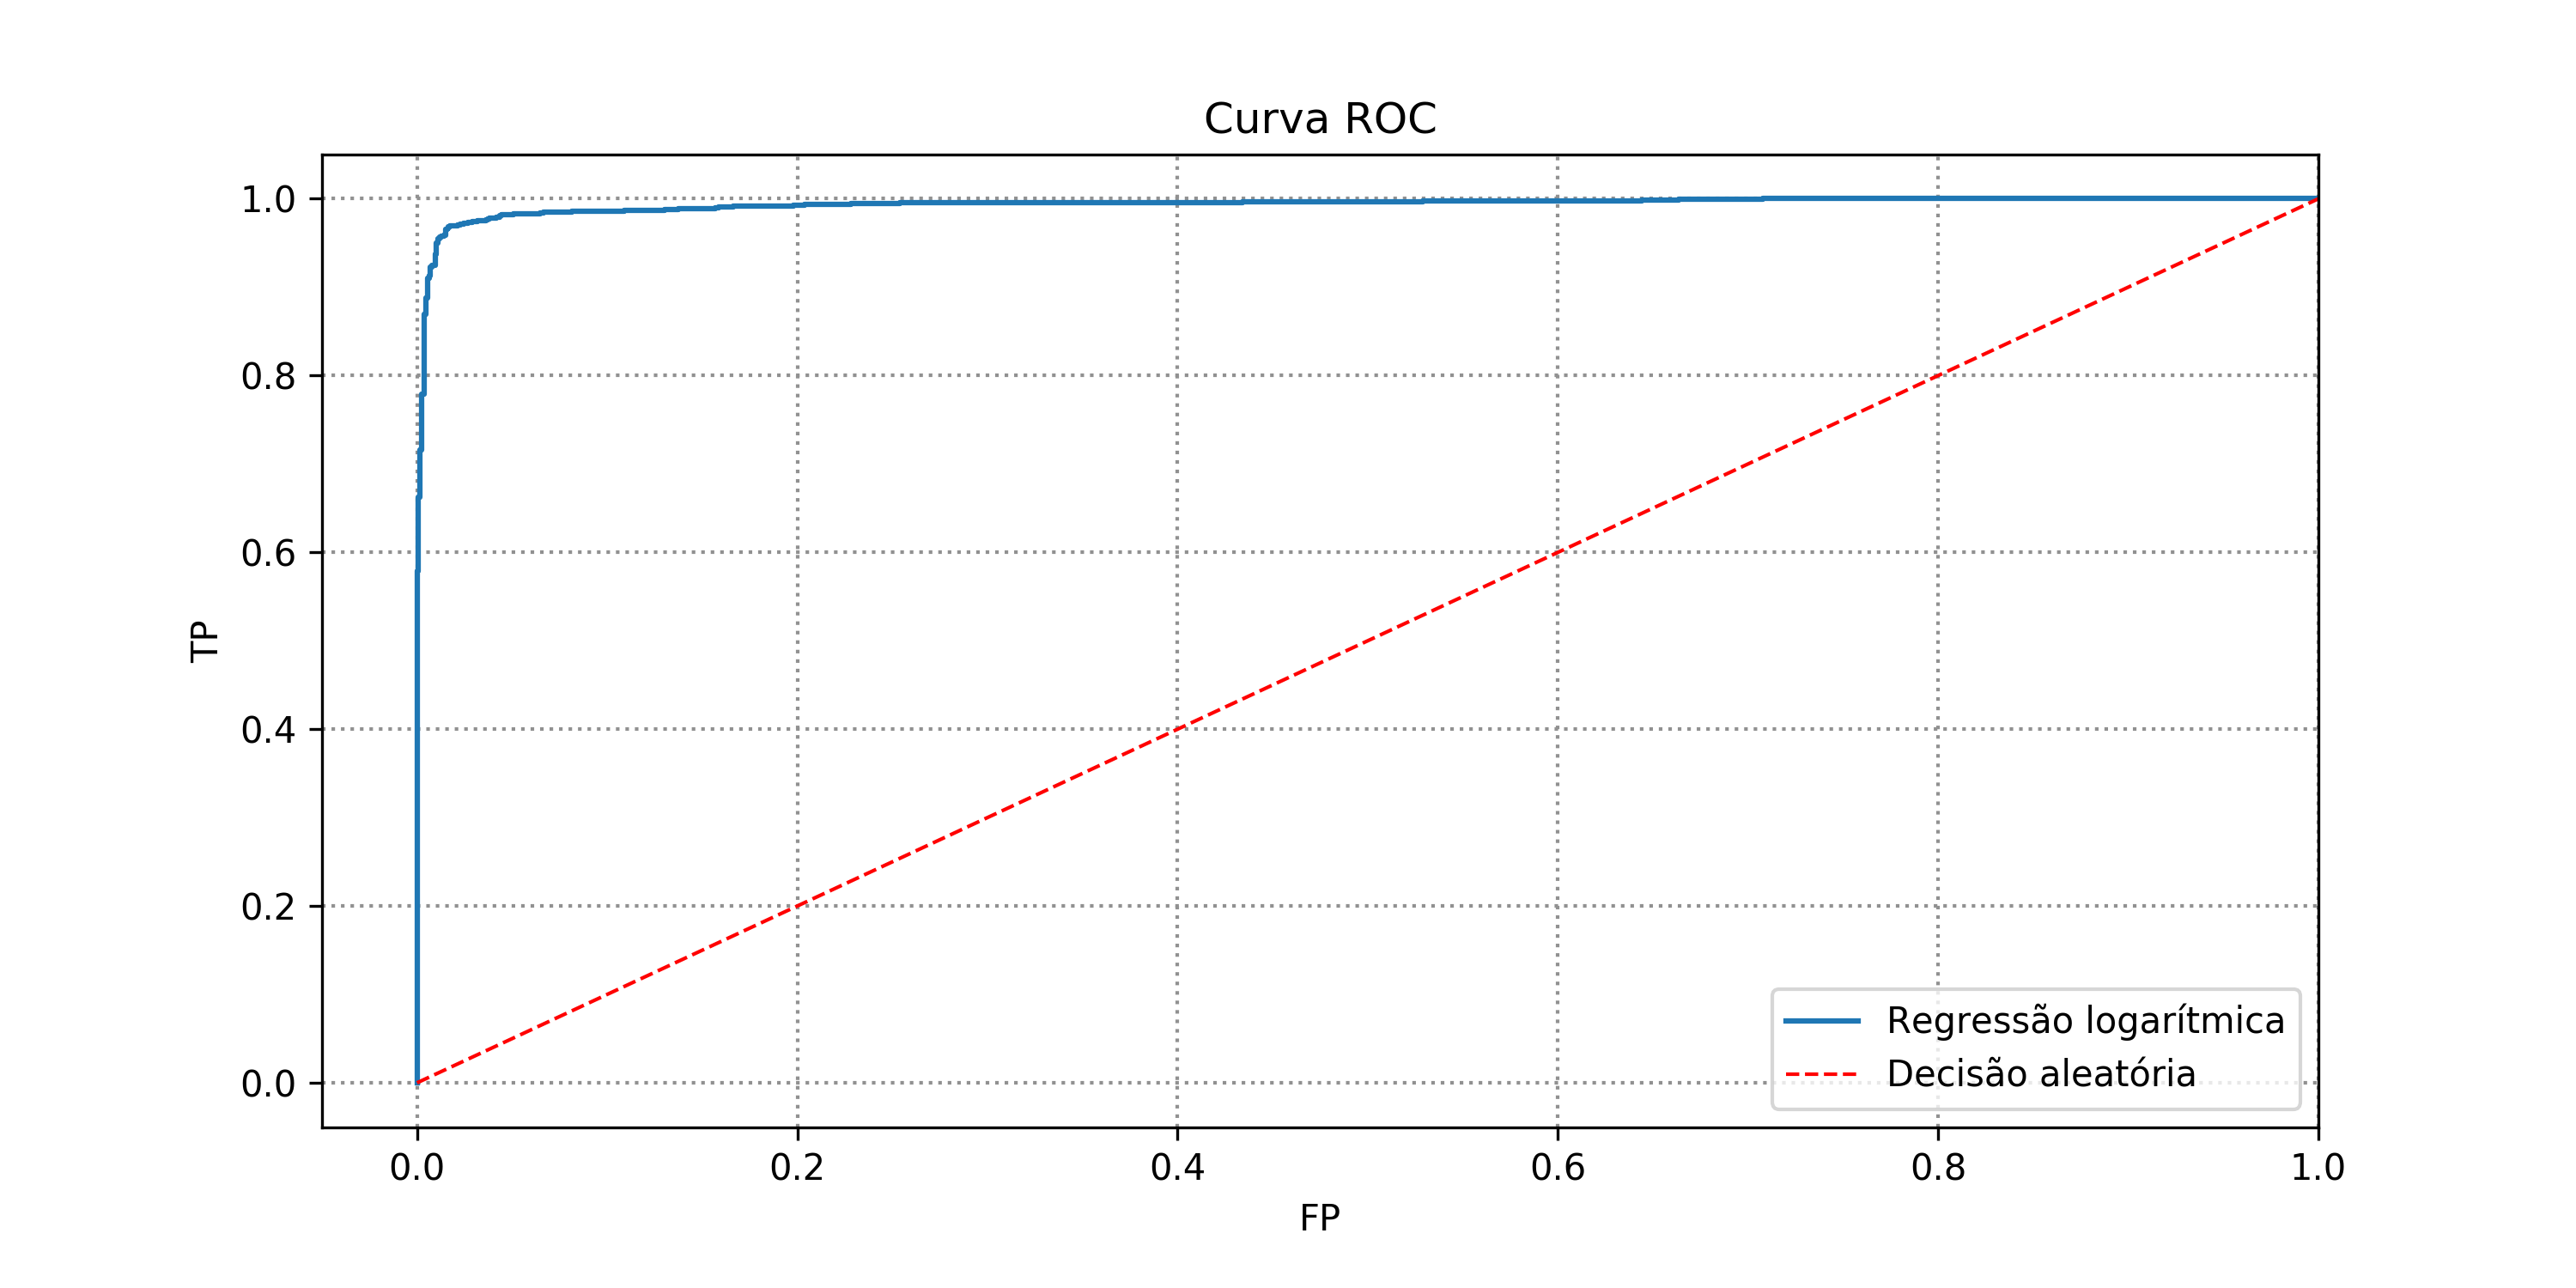
\includegraphics[width=\textwidth]{img1/roc.png}
            \caption{Classificação binária: Curva ROC relativa aos dados de Teste}
            \label{fig:a_roc}
        \end{figure}
        \begin{figure}[H]
            \centering
            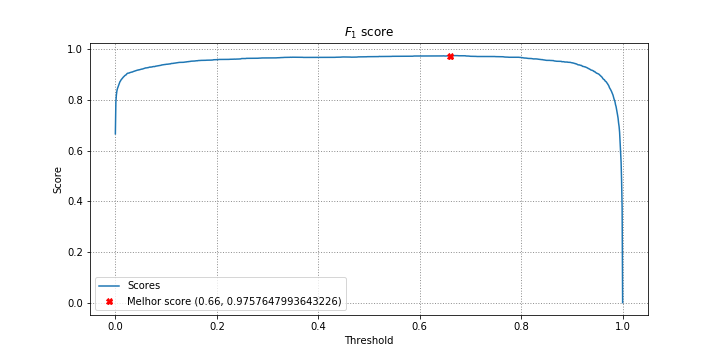
\includegraphics[width=\textwidth]{img1/f1_score.png}
            \caption{Classificação binária: $F_1$-medida relativa aos dados de Teste}
            \label{fig:a_fi_score}
        \end{figure}
    
    \subsection[]{c) Melhor \textit{threshold}, matriz de confusão e acurácia}
    Para a escolha do valor de \textit{threshold} será utilizada a $F_1$-medida, de forma que
    o \textit{recall} e precisão do classificador tenham a mesma importância.

    Conforme apresentado na figura \ref{fig:a_fi_score}, o valor de \textit{threshold} para máxima $F_1$-medida é
    obtido com:
    \begin{align*}
        \textit{threshold}&=0.657 \\
        F_1-medida&\approx0.9757
    \end{align*}
    Utilizando o limiar de máxima $F_1$-medida, a classificação do \textit{dataset} de testes é 
    apresentada conforme a matriz de confusão \ref{ex1_cm}.
    \begin{table}[]
        \begin{tabular}{cccc}
            &  & \multicolumn{2}{c}{\textbf{Classe Estimada}} \\
            &  & Feminino & Masculino \\ \cline{3-4} 
            \textbf{Classe} & \multicolumn{1}{c|}{Feminino} & \multicolumn{1}{c|}{1245} & \multicolumn{1}{c|}{22} \\ \cline{3-4} 
            \textbf{Verdadeira} & \multicolumn{1}{c|}{Masculino} & \multicolumn{1}{c|}{39} & \multicolumn{1}{c|}{1228} \\ \cline{3-4} 
        \end{tabular}
        \caption{Matriz de confusão para o $threshold$ de $0.657$}
        \label{ex1_cm}
    \end{table}
    O classificador apresentou acurácia de aproximadamente $0.975927$. Outras medidas de desempenho como precisão, \textit{recall} e
    $F_1$-medida são apresentadas na tabela \ref{table:ex1_desempenho}. As medidas de desempenho são apresentadas por rótulo (Masculino e Feminino),
    na forma de uma média e como média ponderada pelo número de amostras de cada classe.
    \begin{table}[]
        \begin{tabular}{ccccc}
        \hline
        \textbf{} & \textbf{Precisão} & \textbf{Recall} & \textbf{F1-medida} & \textbf{Amostras} \\ \hline
        \multicolumn{1}{c|}{Feminino} & \multicolumn{1}{c|}{0.969626} & \multicolumn{1}{c|}{0.982636} & \multicolumn{1}{c|}{0.976088} & \multicolumn{1}{c|}{1267} \\ \cline{2-5} 
        \multicolumn{1}{c|}{Masculino} & \multicolumn{1}{c|}{0.982400} & \multicolumn{1}{c|}{0.969219} & \multicolumn{1}{c|}{0.975765} & \multicolumn{1}{c|}{1267} \\ \cline{2-5} 
        \multicolumn{1}{c|}{Média} & \multicolumn{1}{c|}{0.976013} & \multicolumn{1}{c|}{0.975927} & \multicolumn{1}{c|}{0.975926} & \multicolumn{1}{c|}{2534} \\ \cline{2-5} 
        \multicolumn{1}{c|}{Média ponderada} & \multicolumn{1}{c|}{0.976013} & \multicolumn{1}{c|}{0.975927} & \multicolumn{1}{c|}{0.975926} & \multicolumn{1}{c|}{2534} \\ \hline
        \end{tabular}
        \caption{Desempenho do classificador para o $threshold$ de $0.657$}
        \label{table:ex1_desempenho}
    \end{table}
    
    \section[]{Parte 2 – Classificação multi-classe}
    Será abordado um problema de classificação multi-classe com $6$ rótulos, conforme a tabela \ref{table:ex2_rotulos}, e $561$ atributos.
    \begin{table}[]
        \begin{tabular}{|c|c|c|c|c|c|}
        \hline
        0 & 1 & 2 & 3 & 4 & \textbf{5} \\ \hline
        \textbf{Caminhada} & \textbf{Subindo Escadas} & \textbf{Descendo Escadas} & \textbf{Sentado} & \textbf{Em pé} & \textbf{Deitado} \\ \hline
        \end{tabular}
        \caption{Rótulos}
        \label{table:ex2_rotulos}
    \end{table}
    \subsection[]{a) Regressão logística}
    Para a classificação multi-classe é adotada a \textit{softmax}, sendo gerado um modelo capaz de produzir $Q$
    saídas que representam a probabilidade do padão apresentado pertencer a uma classe específica. Tal modelo apresenta
    maior robustez que as abordagens um-contra-todos e um-contra-um.

    Na etapa de pré-processamento dos dados, o \textit{dataset} de entrada foi normalizado utilizando a $z-score$ e os rótulos (\textit{dataset} de saída)
    transformados com o processo de \textit{one hot encoding}.
    O processo de treinamento do modelo foi finalizado com o modelo classificando corretamente $98,89\%$ dos padrões de treinamento.

    A matriz de confusão apresentada na tabela \ref{table:ex2_cm_softmax} foi obtida com o teste do modelo.
    \begin{table}[]
        \begin{tabular}{ccccccc}
        & \textbf{Caminhada} & \textbf{\begin{tabular}[c]{@{}c@{}}Subindo\\ Escadas\end{tabular}} & \textbf{\begin{tabular}[c]{@{}c@{}}Descendo\\ Escadas\end{tabular}} & \textbf{Sentado} & \textbf{Em pé} & \textbf{Deitado} \\ \cline{2-7} 
        \multicolumn{1}{c|}{\textbf{Caminhada}} & \multicolumn{1}{c|}{479} & \multicolumn{1}{c|}{8} & \multicolumn{1}{c|}{9} & \multicolumn{1}{c|}{0} & \multicolumn{1}{c|}{0} & \multicolumn{1}{c|}{0} \\ \cline{2-7} 
        \multicolumn{1}{c|}{\textbf{\begin{tabular}[c]{@{}c@{}}Subindo\\ Escadas\end{tabular}}} & \multicolumn{1}{c|}{8} & \multicolumn{1}{c|}{460} & \multicolumn{1}{c|}{3} & \multicolumn{1}{c|}{0} & \multicolumn{1}{c|}{0} & \multicolumn{1}{c|}{0} \\ \cline{2-7} 
        \multicolumn{1}{c|}{\textbf{\begin{tabular}[c]{@{}c@{}}Descendo\\ Escadas\end{tabular}}} & \multicolumn{1}{c|}{11} & \multicolumn{1}{c|}{33} & \multicolumn{1}{c|}{376} & \multicolumn{1}{c|}{0} & \multicolumn{1}{c|}{0} & \multicolumn{1}{c|}{0} \\ \cline{2-7} 
        \multicolumn{1}{c|}{\textbf{Sentado}} & \multicolumn{1}{c|}{0} & \multicolumn{1}{c|}{2} & \multicolumn{1}{c|}{0} & \multicolumn{1}{c|}{428} & \multicolumn{1}{c|}{58} & \multicolumn{1}{c|}{3} \\ \cline{2-7} 
        \multicolumn{1}{c|}{\textbf{Em pé}} & \multicolumn{1}{c|}{0} & \multicolumn{1}{c|}{0} & \multicolumn{1}{c|}{0} & \multicolumn{1}{c|}{16} & \multicolumn{1}{c|}{516} & \multicolumn{1}{c|}{0} \\ \cline{2-7} 
        \multicolumn{1}{c|}{\textbf{Deitado}} & \multicolumn{1}{c|}{0} & \multicolumn{1}{c|}{0} & \multicolumn{1}{c|}{0} & \multicolumn{1}{c|}{0} & \multicolumn{1}{c|}{24} & \multicolumn{1}{c|}{513} \\ \cline{2-7} 
        \end{tabular}
        \caption{Matriz de confusão, \textit{dataset} testes com o modelo explorando a função \textit{softmax}}
        \label{table:ex2_cm_softmax}
    \end{table}

    \begin{table}[]
    \begin{tabular}{ccccc}
        & \textbf{Precisão} & \textbf{Recall} & \textbf{F1-medida} & \textbf{Medidas} \\ \cline{2-5} 
        \multicolumn{1}{c|}{\textbf{Caminhada}} & \multicolumn{1}{c|}{0.961847} & \multicolumn{1}{c|}{0.965726} & \multicolumn{1}{c|}{0.963783} & \multicolumn{1}{c|}{496} \\ \cline{2-5} 
        \multicolumn{1}{c|}{\textbf{\begin{tabular}[c]{@{}c@{}}Subindo\\ Escadas\end{tabular}}} & \multicolumn{1}{c|}{0.914513} & \multicolumn{1}{c|}{0.976645} & \multicolumn{1}{c|}{0.944559} & \multicolumn{1}{c|}{471} \\ \cline{2-5} 
        \multicolumn{1}{c|}{\textbf{\begin{tabular}[c]{@{}c@{}}Descendo\\ Escadas\end{tabular}}} & \multicolumn{1}{c|}{0.969072} & \multicolumn{1}{c|}{0.895238} & \multicolumn{1}{c|}{0.930693} & \multicolumn{1}{c|}{420} \\ \cline{2-5} 
        \multicolumn{1}{c|}{\textbf{Sentado}} & \multicolumn{1}{c|}{0.963964} & \multicolumn{1}{c|}{0.871690} & \multicolumn{1}{c|}{0.915508} & \multicolumn{1}{c|}{491} \\ \cline{2-5} 
        \multicolumn{1}{c|}{\textbf{Em pé}} & \multicolumn{1}{c|}{0.862876} & \multicolumn{1}{c|}{0.969925} & \multicolumn{1}{c|}{0.913274} & \multicolumn{1}{c|}{532} \\ \cline{2-5} 
        \multicolumn{1}{c|}{\textbf{Deitado}} & \multicolumn{1}{c|}{0.994186} & \multicolumn{1}{c|}{0.955307} & \multicolumn{1}{c|}{0.974359} & \multicolumn{1}{c|}{537} \\ \cline{2-5} 
        &  &  &  &  \\ \cline{2-5} 
        \multicolumn{1}{c|}{\textbf{Acurácia}} & \multicolumn{1}{c|}{} & \multicolumn{1}{c|}{} & \multicolumn{1}{c|}{0.940618} & \multicolumn{1}{c|}{2947} \\ \cline{2-5} 
        \multicolumn{1}{c|}{\textbf{Média macro}} & \multicolumn{1}{c|}{0.944410} & \multicolumn{1}{c|}{0.939089} & \multicolumn{1}{c|}{0.940363} & \multicolumn{1}{c|}{2947} \\ \cline{2-5} 
        \multicolumn{1}{c|}{\textbf{Média ponderada}} & \multicolumn{1}{c|}{0.943691} & \multicolumn{1}{c|}{0.940618} & \multicolumn{1}{c|}{0.940761} & \multicolumn{1}{c|}{2947} \\ \cline{2-5} 
        \end{tabular}
    \caption{Métricas de desempenho do classificador}
    \label{table:ex2_desempenho}
    \end{table}
    Será adotada como métrica para avaliação de desempenho a $F_1-score$ macro, por dar a mesmam importância para a precisão e o 
    \textit{recall} do estimador e pelo tratamento igualitário a todas as classes.
    
    \subsection[]{b) kNN}
    Para o uso do kNN, os \textit{datasets} de entrada são normalizados utilizando a $z-score$ e o melhor valor para o número de 
    vizinhos $k$ é encontrado com o uso da técnica de validação cruzada $K-Fold$, com $5$ folds. 

    O melhor resultado de classificação na validação cruzada é obtido com $k=26$ vizinhos, conforme é mostrado no gráfico \ref{fig:ex2_b_knn}.
    A figura \ref{fig:ex2_b_knn} apresenta o valor médio da quantidade de estimações incorretas obtidos nos $5$ folds para $k$ vizinhos.
    \begin{figure}[H]
        \centering
        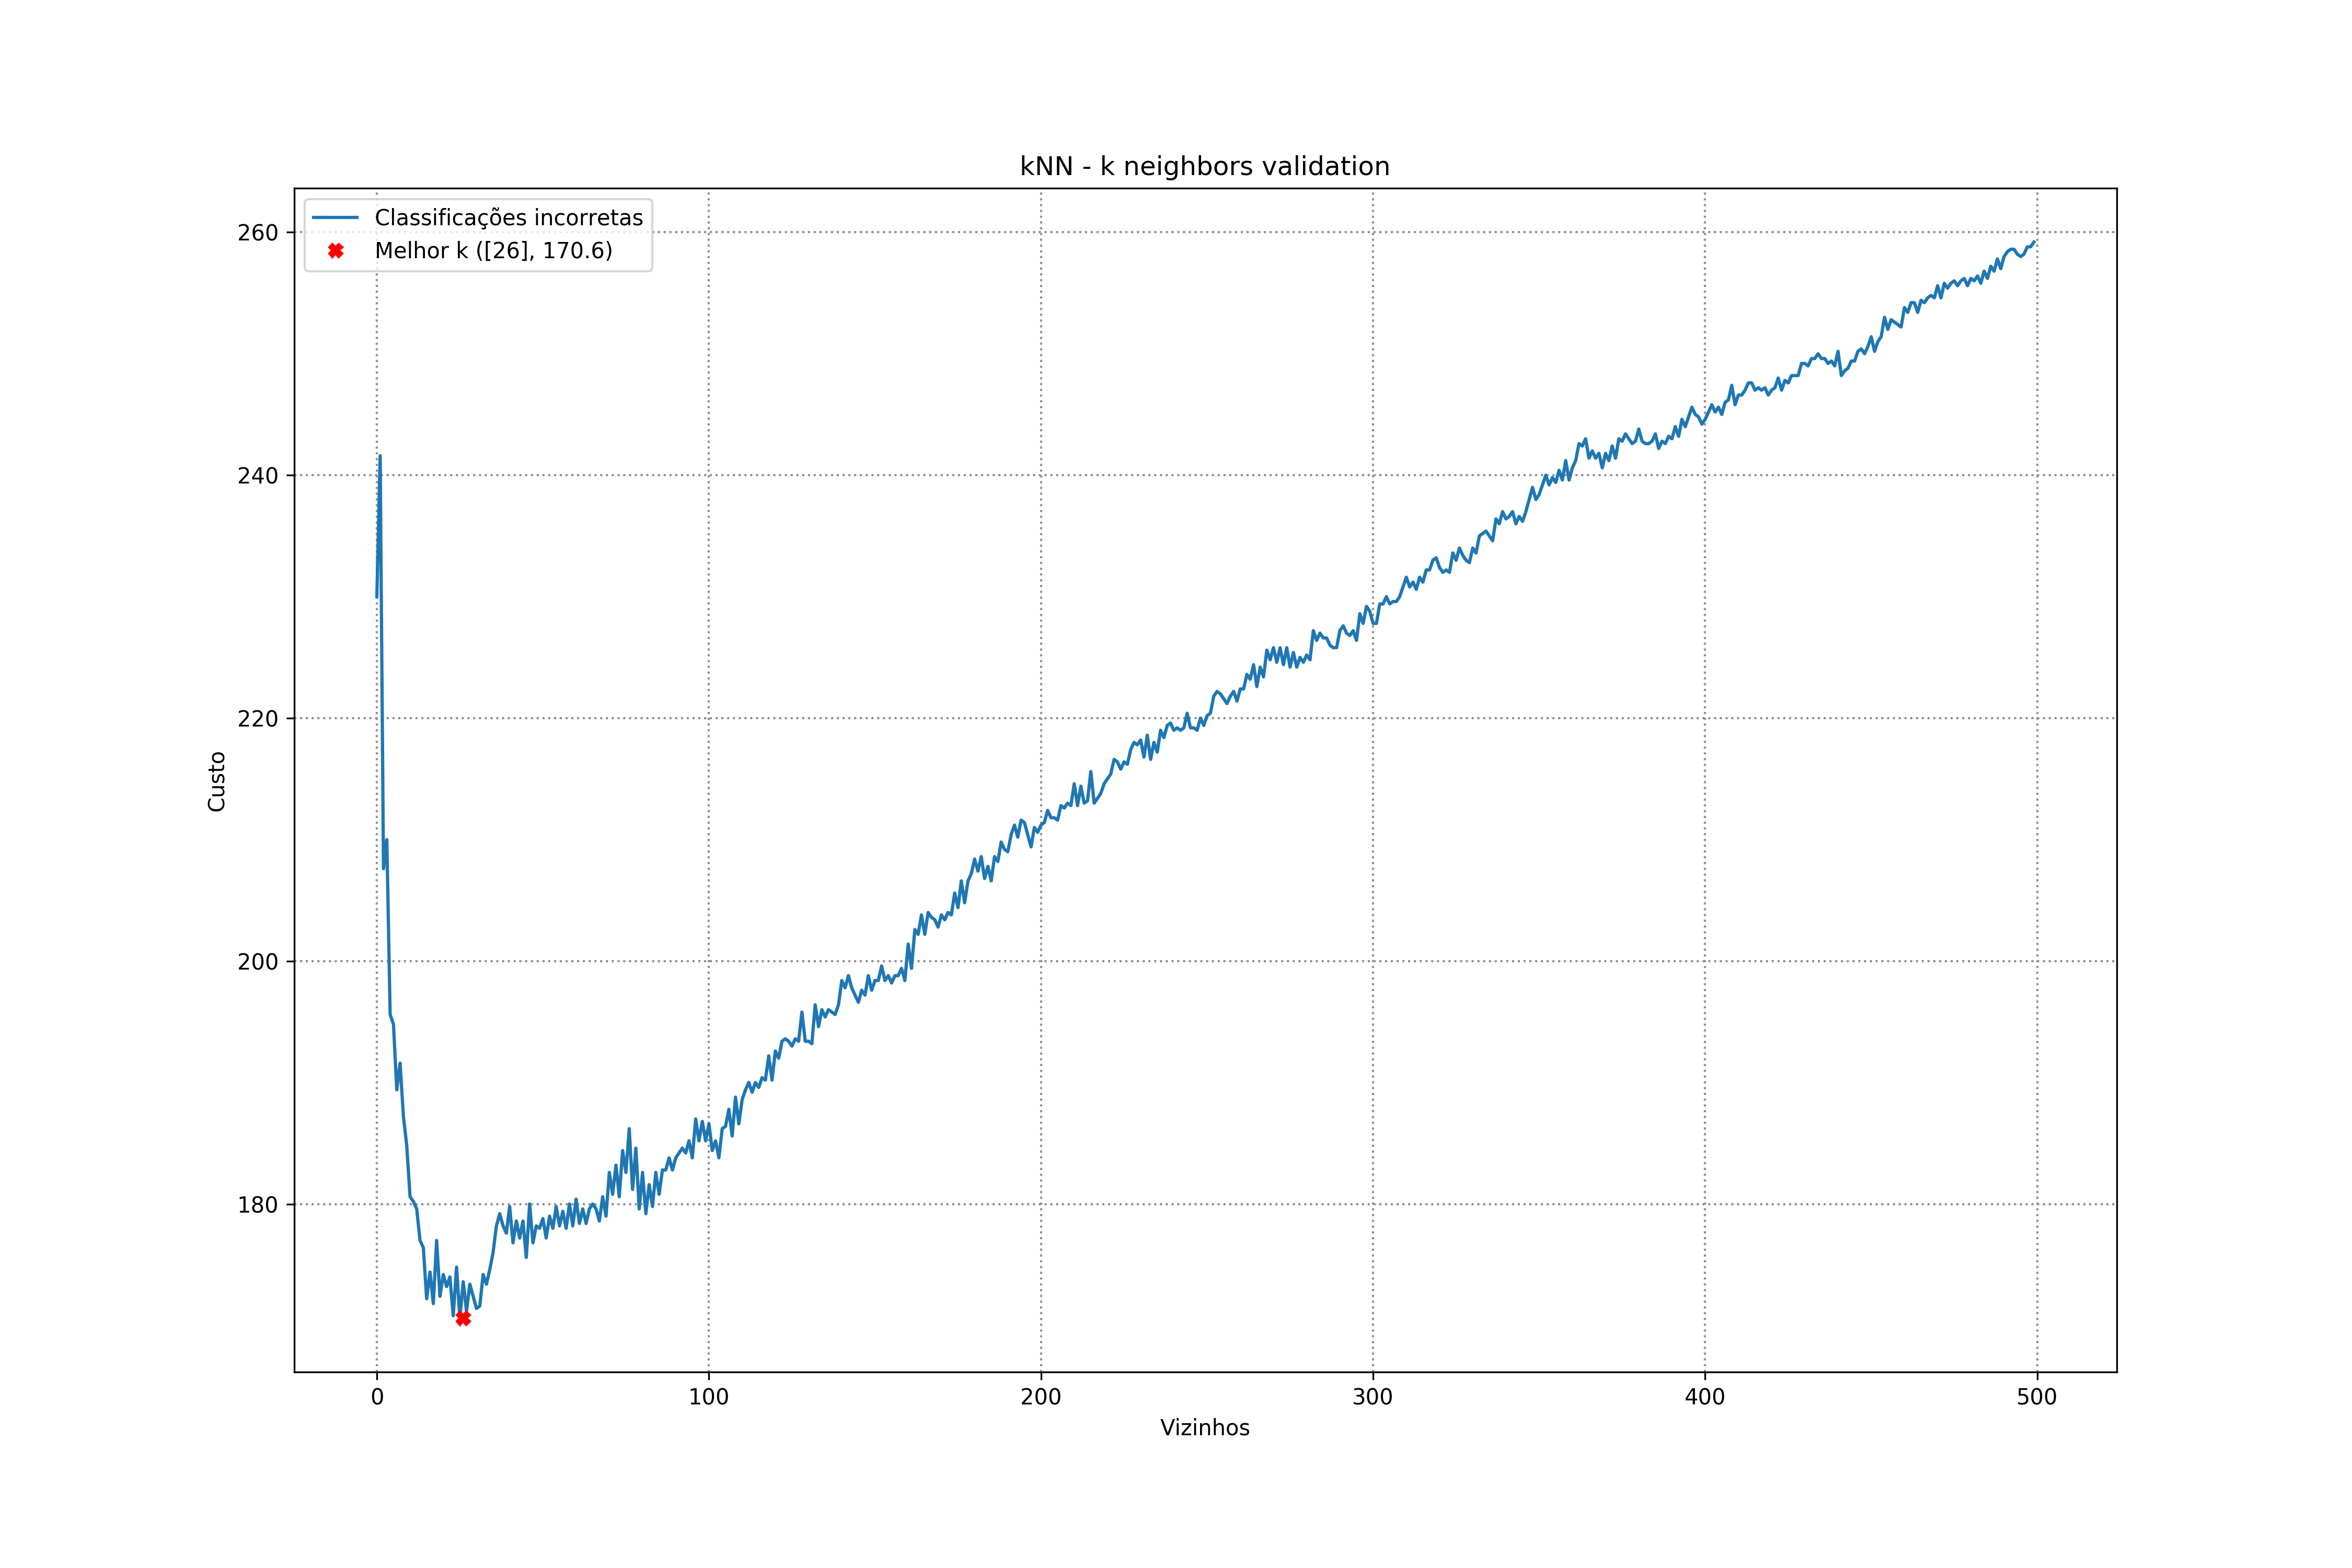
\includegraphics[width=.8\linewidth]{img2/knn.png}
        \caption{kNN: Média das estimações incorretas dos $K-Folds$ para $k$ vizinhos}
        \label{fig:ex2_b_knn}
    \end{figure}

    Ao término da etapa de testes é obtida a matriz de confusão \ref{table:ex2_knn_cm}.

    \begin{table}[H]
        \begin{tabular}{ccccccc}
        & \textbf{Caminhada} & \textbf{\begin{tabular}[c]{@{}c@{}}Subindo\\ Escadas\end{tabular}} & \textbf{\begin{tabular}[c]{@{}c@{}}Descendo\\ Escadas\end{tabular}} & \textbf{Sentado} & \textbf{Em pé} & \textbf{Deitado} \\ \cline{2-7} 
        \multicolumn{1}{c|}{\textbf{Caminhada}} & \multicolumn{1}{c|}{489} & \multicolumn{1}{c|}{2} & \multicolumn{1}{c|}{5} & \multicolumn{1}{c|}{0} & \multicolumn{1}{c|}{0} & \multicolumn{1}{c|}{0} \\ \cline{2-7} 
        \multicolumn{1}{c|}{\textbf{\begin{tabular}[c]{@{}c@{}}Subindo\\ Escadas\end{tabular}}} & \multicolumn{1}{c|}{49} & \multicolumn{1}{c|}{419} & \multicolumn{1}{c|}{3} & \multicolumn{1}{c|}{0}  & \multicolumn{1}{c|}{0} & \multicolumn{1}{c|}{0} \\ \cline{2-7} 
        \multicolumn{1}{c|}{\textbf{\begin{tabular}[c]{@{}c@{}}Descendo\\ Escadas\end{tabular}}} & \multicolumn{1}{c|}{67} & \multicolumn{1}{c|}{59} & \multicolumn{1}{c|}{294} & \multicolumn{1}{c|}{0} & \multicolumn{1}{c|}{0} & \multicolumn{1}{c|}{0} \\ \cline{2-7} 
        \multicolumn{1}{c|}{\textbf{Sentado}} & \multicolumn{1}{c|}{0} & \multicolumn{1}{c|}{2} & \multicolumn{1}{c|}{0} & \multicolumn{1}{c|}{387} & \multicolumn{1}{c|}{100} & \multicolumn{1}{c|}{2} \\ \cline{2-7} 
        \multicolumn{1}{c|}{\textbf{Em pé}} & \multicolumn{1}{c|}{0} & \multicolumn{1}{c|}{0} & \multicolumn{1}{c|}{0} & \multicolumn{1}{c|}{21} & \multicolumn{1}{c|}{511} & \multicolumn{1}{c|}{0} \\ \cline{2-7} 
        \multicolumn{1}{c|}{\textbf{Deitado}} & \multicolumn{1}{c|}{0} & \multicolumn{1}{c|}{0} & \multicolumn{1}{c|}{0} & \multicolumn{1}{c|}{10} & \multicolumn{1}{c|}{18} & \multicolumn{1}{c|}{509} \\ \cline{2-7} 
        \end{tabular}
        \caption{kNN: Matriz de confusão}
        \label{table:ex2_knn_cm}
    \end{table}

    Os
    \begin{table}[H]
        \begin{tabular}{ccccc}
        & \textbf{Precisão} & \textbf{Recall} & \textbf{F1-medida} & \textbf{Medidas} \\ \cline{2-5} 
        \multicolumn{1}{c|}{\textbf{Caminhada}} & \multicolumn{1}{c|}{0.808264} & \multicolumn{1}{c|}{0.985887} & \multicolumn{1}{c|}{0.888283} & \multicolumn{1}{c|}{496} \\ \cline{2-5} 
        \multicolumn{1}{c|}{\textbf{\begin{tabular}[c]{@{}c@{}}Subindo\\ Escadas\end{tabular}}} & \multicolumn{1}{c|}{0.869295} & \multicolumn{1}{c|}{0.889597} & \multicolumn{1}{c|}{0.879328} & \multicolumn{1}{c|}{471} \\ \cline{2-5} 
        \multicolumn{1}{c|}{\textbf{\begin{tabular}[c]{@{}c@{}}Descendo\\ Escadas\end{tabular}}} & \multicolumn{1}{c|}{0.973510} & \multicolumn{1}{c|}{0.700000} & \multicolumn{1}{c|}{0.814404} & \multicolumn{1}{c|}{420} \\ \cline{2-5} 
        \multicolumn{1}{c|}{\textbf{Sentado}} & \multicolumn{1}{c|}{0.925837} & \multicolumn{1}{c|}{0.788187} & \multicolumn{1}{c|}{0.851485} & \multicolumn{1}{c|}{491} \\ \cline{2-5} 
        \multicolumn{1}{c|}{\textbf{Em pé}} & \multicolumn{1}{c|}{0.812401} & \multicolumn{1}{c|}{0.960526} & \multicolumn{1}{c|}{0.880276} & \multicolumn{1}{c|}{532} \\ \cline{2-5} 
        \multicolumn{1}{c|}{\textbf{Deitado}} & \multicolumn{1}{c|}{0.996086} & \multicolumn{1}{c|}{0.947858} & \multicolumn{1}{c|}{0.971374} & \multicolumn{1}{c|}{537} \\ \cline{2-5} 
        &  &  &  &  \\ \cline{2-5} 
        \multicolumn{1}{c|}{\textbf{Acurácia}} & \multicolumn{1}{c|}{} & \multicolumn{1}{c|}{} & \multicolumn{1}{c|}{0.885307} & \multicolumn{1}{c|}{2947} \\ \cline{2-5} 
        \multicolumn{1}{c|}{\textbf{Média macro}} & \multicolumn{1}{c|}{0.897566} & \multicolumn{1}{c|}{0.878676} & \multicolumn{1}{c|}{\cellcolor[HTML]{DAE8FC}0.880859} & \multicolumn{1}{c|}{2947} \\ \cline{2-5} 
        \multicolumn{1}{c|}{\textbf{Média ponderada}} & \multicolumn{1}{c|}{0.896129} & \multicolumn{1}{c|}{0.885307} & \multicolumn{1}{c|}{0.883887} & \multicolumn{1}{c|}{2947} \\ \cline{2-5} 
        \end{tabular}
        \caption{kNN: Métricas de desempenho na etapa de testes}
        \label{table:ex2_knn_desempenho}
    \end{table}

\end{document}